\documentclass[
    english,
    ruledheaders=section,
    class=report,
    thesis={type=bachelor},
    accentcolor=2c,
    custommargins=false,
    marginpar=false,
    parskip=half-,
    fontsize=11pt,
    IMRAD=false,
    bibliography=totoc,
]{tudapub}

\usepackage[main=english]{babel}
\usepackage{biblatex}
\addbibresource{thesis.bib}
\usepackage{csquotes}
\usepackage{stmaryrd, amsmath, amssymb, amsfonts, amsthm}
\usepackage{multicol}
\usepackage{mathtools}
\usepackage{bussproofs}
\usepackage{xcolor}
\usepackage{mathrsfs}
\usepackage{xspace}
\usepackage{paralist}
\usepackage{nicefrac}
\usepackage{multirow}
\usepackage{hyperref}
\usepackage{tikz}
\usetikzlibrary{calc,trees,decorations,arrows,automata,positioning,plotmarks, shapes,shapes.geometric,backgrounds}
\newcommand{\Bool}[0]{\operatorname{Bool}}
\newcommand{\True}[0]{\operatorname{true}}
\newcommand{\False}[0]{\operatorname{false}}
\newcommand{\Maybe}[1]{\operatorname{Maybe}\; #1}
\newcommand{\Just}[1]{\operatorname{Just}\; #1}
\newcommand{\Nothing}[0]{\operatorname{Nothing}}
\newcommand{\Or}[0]{\; | \;}
\newcommand{\Promise}[1]{\operatorname{Promise}\; #1}
\newcommand{\Proposal}[1]{\operatorname{Proposal}\; #1}
\newcommand{\ProposalC}[2]{\operatorname{Proposal}\; #1\; #2}
\newcommand{\Nack}[1]{\operatorname{Nack}\; #1}
\newcommand{\Value}[0]{\operatorname{Value}}

\newcommand{\Curly}[1]{\left\{#1\right\}}
\newcommand{\Paren}[1]{\left(#1\right)}

\newcommand{\DotForall}[1]{\bigodot_{#1}\;}
\newcommand{\SendUnreliableG}[4]{#1 \to_u #2 : #3 \left\langle #4 \right\rangle}
\newcommand{\SendWeaklyG}[3]{#1 \to_w #2 : #3}

\newcommand{\Accept}[0]{\mathnormal{Accept}}
\newcommand{\Restart}[0]{\mathnormal{Restart}}
\newcommand{\Abort}[0]{\mathnormal{Abort}}

\newcommand{\Mu}[1]{\left(\mu #1\right)}

\newcommand{\prNumber}[2]{\operatorname{proposalNumber}\left( #1, #2 \right)}
\newcommand{\promValue}[1]{\operatorname{promiseValue}\left(#1\right)}
\newcommand{\anyNack}[1]{\operatorname{anyNack}\left(#1\right)}
\newcommand{\promiseCount}[1]{\operatorname{promiseCount}\left(#1\right)}
\newcommand{\greaterThan}[2]{\operatorname{gt}\left(#1, #2\right)}
\newcommand{\greaterEqual}[2]{\operatorname{ge}\left(#1, #2\right)}
\newcommand{\nFromProposal}[1]{\operatorname{nFromProposal}\left(#1 \right)}
\newcommand{\genAq}[3]{\operatorname{genA_Q}\left(#1, #2, #3\right)}
\newcommand{\update}[2]{\operatorname{update} \left(#1, #2\right)}

\newcommand{\Sys}[2]{\operatorname{Sys}\left(#1, #2\right)}
\newcommand{\Pa}[0]{\operatorname{P^a}}
\newcommand{\Pp}[0]{\operatorname{P^p}}
\newcommand{\PaCont}[0]{\operatorname{P^a_{cont}}}

\newcommand{\PpInit}[5]{\operatorname{P^p_{init}}\left(#1, #2, #3, #4, #5\right)}
\newcommand{\PaInit}[6]{\operatorname{P^a_{init}}\left(#1, #2, #3, #4, #5, #6\right)}

\newcommand{\SessionRequest}[3]{\overline{#1}\left[#2\right]\left(#3\right)}
\newcommand{\SessionAccept}[3]{#1\left[#2\right]\left(#3\right)}
\newcommand{\ParallelFor}[1]{\Pi_{#1}\;}
\newcommand{\VectorV}[0]{\overrightarrow{V}}

\newcommand{\SendUnreliableP}[5]{#1\left[#2, #3\right]!_u #4 \left\langle #5 \right\rangle}
\newcommand{\ReceiveUnreliableP}[6]{#1\left[#2, #3\right]?_u #4 \left\langle #5 \right\rangle \left(#6\right)}
\newcommand{\ceil}[1]{\Big\lceil #1 \Big\rceil}
\newcommand{\SendWeaklyP}[5]{#1\left[#2, #3\right]!_w #4.#5}
\newcommand{\ReceiveWeaklyP}[4]{#1\left[#2, #3\right]?_w #4}
\newcommand{\If}[1]{\operatorname{if}\; #1}
\newcommand{\Then}[1]{\operatorname{then}\; #1}
\newcommand{\Else}[1]{\operatorname{else}\; #1}
\newcommand{\tOr}[0]{\text{ or }}

\newcommand{\FPuget}[0]{\mathtt{FP_{uget}}}
\newcommand{\FPuskip}[0]{\mathtt{FP_{uskip}}}
\newcommand{\FPml}[0]{\mathtt{FP_{ml}}}
\newcommand{\FPwskip}[0]{\mathtt{FP_{wskip}}}
\newcommand{\FPcrash}[0]{\mathtt{FP_{crash}}}
\newcommand{\EventuallyWeak}[0]{\Diamond\mathscr{W}}

\newcommand{\Nu}[1]{\left(\nu #1\right)}
\newcommand{\OuterSessionQueues}[0]{\ParallelFor{1 \le k,l \le 2, k \neq l} t_{k\to l}:[]}
\newcommand{\InnerSessionQueues}[1]{\ParallelFor{1 \le k,l \le 4, k \neq l} #1_{k\to l}:[]}
\newcommand{\NuChannels}[0]{\Nu{t}\Nu{s}\Nu{r}}

\newcommand{\BeginPaCont}[0]{\Accept \dots \oplus \Restart .X \oplus \Abort .end}
\newcommand{\ABC}[0]{\operatorname{abc}}
\newcommand{\Acceptor}[1]{\operatorname{A_#1}}
\newcommand{\Proposer}[1]{\operatorname{P_#1}}

\newcommand{\Init}[0]{\Paren{\operatorname{Init}}}
\newcommand{\comment}[1]{\;\textcolor{teal}{#1}}

\newcommand{\Usend}[0]{\Paren{\operatorname{USend}}}
\newcommand{\Uget}[0]{\Paren{\operatorname{UGet}}}
\newcommand{\Uskip}[0]{\Paren{\operatorname{USkip}}}
\newcommand{\Wsel}[0]{\Paren{\operatorname{WSel}}}
\newcommand{\Wbran}[0]{\Paren{\operatorname{WBran}}}
\newcommand{\Wskip}[0]{\Paren{\operatorname{WSkip}}}

\begin{document}
\title{Analyzing Paxos with Fault-Tolerant Multiparty Session Types}
\author[N. D. Torres]{Nicolas Daniel Torres}
\department{inf}
\group{Theory of Parallel Systems}
\reviewer{Prof. Dr. Kirstin Peters \and M.Sc. Anna Schmitt}
\submissiondate{\today}
\maketitle
\affidavit[signature-image={\includegraphics[width=\width,height=2cm]{Unterschrift.png}}, affidavit=digital]

\chapter*{Abstract}
Achieving consensus among multiple, possibly faulty and unreliable processes is a fundamental problem in distributed computing.
In order to solve this consensus problem, consensus algorithms like Paxos must satisfy validity, agreement, and termination.
Proving these properties can be complicated.
Static analysis is preferable because model checking tools lead to big state-spaces.
Our aim in this work is to apply Fault-Tolerant Multiparty Session Types -- a fault-tolerant extension to Multiparty Session Types -- to statically analyze a consensus algorithm.
We construct a model of Paxos, including its fault-tolerant aspects.
Static analysis of that model helps us prove validity, agreement, and termination for it.


\tableofcontents

% \IMRADlabel{introduction}
\chapter{Introduction}

% coordinating processes?
% - processes that need to achieve one goal together
% - accessing shared data
% - ensure correct (distributed) computation
% - reliable distributed coordination
In distributed computing, it is often necessary for coordinating processes to reach consensus, i.e., agree on the value of some data that are needed during computation.
These processes agree on the same values to ensure correct computation, which necessitates a correct consensus algorithm.
Thus, proving the correctness of consensus algorithms is important.

Due to the presence of faulty processes consensus algorithms are designed to be fault-tolerant.
To achieve fault-tolerance these algorithms must satisfy the following properties: termination, integrity, and agreement\cite{dist_sys}.

Proving these properties can be complicated.
Dynamic analysis tools lead to big state-spaces so static analysis is preferable.
Multiparty Session Types are particularly interesting since session typing can ensure absence of communication errors and deadlocks, and protocol conformance\cite{mpstbd}.
However, to properly model unreliable communication between processes a fault-tolerant extension to Multiparty Session Types is necessary.

\citeauthor{ftmpst} developed such an extension.


% \IMRADlabel{methods}
\chapter{Technical Preliminaries}
\label{chapter:technicalpreliminaries}
% In this chapter we will introduce the Paxos consensus algorithm, Multiparty Session Types (\MPST), Fault-Tolerant Multiparty Session Types (\FTMPST), and some notation.
% FTMPST, Paxos, Some Notation
\section{Paxos}
\citeauthor{Lamport01} describes the Paxos algorithm in \cite{Lamport01}.
First, he outlines the problem and then the algorithm to solve that problem.

\subsection{The Problem}
Assume a collection of processes that can propose values.
A consensus algorithm ensures that a single one among the proposed values is chosen.
If no value is proposed, then no value should be chosen.
If a value has been chosen, then processes should be able to learn the chosen value.
The safety requirements for consensus are:

\begin{itemize}
    % Validity
    \item \textbf{Validity}: Only a value that has been proposed may be chosen,
    % Agreement
    \item \textbf{Agreement}: Only a single value is chosen, and
    % Termination? I'd prefer
    % "If a value has been proposed and sufficient processes remain non-faulty, then eventually some value is chosen."
    % \item A process never learns that a value has been chosen unless it actually has been.
    \item \textbf{Termination}: If a value has been proposed and sufficient processes remain non-faulty, then eventually some value is chosen (compare to \cite{Lamport05}).
\end{itemize}

% TODO "These are the properties we will prove with the model" oder sowas in der Art.

Assume that agents can communicate with one another by sending messages.
We use the customary asynchronous, non-Byzantine model, in which:

\begin{itemize}
    \item Agents operate at arbitrary speed, may fail by stopping, and may restart.
    Since all agents may fail after a value is chosen and then restart, a solution is impossible unless some information can be remembered by an agent that has failed and restarted.
    \item Messages can take arbitrarily long to be delivered, can be duplicated, and can be lost, but they are not corrupted.
\end{itemize}

We assume two classes of agents: proposers and acceptors.

A \emph{quorum} is a set of acceptors that can choose a value proposed by a proposer \cite{Lamport06}.
In Paxos, a quorum is a majority of acceptors.

\subsection{The Algorithm}

\begin{phase}
    $(a)$ A proposer selects a proposal number $n$ and sends a \emph{prepare} request with number $n$ to a majority of acceptors.
    
    $(b)$ If an acceptor receives a \emph{prepare} request with number $n$ greater than that of any \emph{prepare} request to which it has already responded, then it responds to the request with a promise not to accept any more proposals numbered less than $n$ and with the highest-numbered proposal (if any) that it has accepted.
\end{phase}

\begin{phase}
    $(a)$ If the proposer receives a response to its \emph{prepare} requests (numbered $n$) from a majority of acceptors, then it sends an \emph{accept} request to each of those acceptors for a proposal numbered $n$ with a value $v$, where $v$ is the value of the highest-numbered proposal among the responses, or is any value if the responses reported no proposals.

    $(b)$ If an acceptor receives an \emph{accept} request for a proposal numbered $n$, it accepts the proposal unless it has already responded to a \emph{prepare} request having a number greater than $n$.
\end{phase}

A proposer can make multiple proposals, so long as it follows the algorithm for each one.
It can abandon a proposal in the middle of the protocol at any time.
It is probably a good idea to abandon a proposal if some proposer has begun trying to issue a higher-numbered one.
Therefore, if an acceptor ignores a \emph{prepare} or \emph{accept} request because it has already received a \emph{prepare} request with a higher number, then it should probably inform the proposer, who should then abandon its proposal.
This is a performance optimization that does not affect correctness.

To guarantee progress, a distinguished proposer must be selected as the only one to try issuing proposals.
If the distinguished proposer can communicate successfully with a majority of acceptors, and if it uses a proposal with number greater than any already used, then it will succeed in issuing a proposal that is accepted.
By abandoning a proposal and trying again if it learns about some request with a higher proposal number, the distinguished proposer will eventually choose a high enough proposal number.

If enough of the system is working properly, liveness can therefore be achieved by electing a single distinguished proposer.

\subsection{The Implementation}
The Paxos algorithm \cite{Lamport98} assumes a network of processes.
In its consensus algorithm, each process plays the role of proposer, acceptor.
The algorithm chooses a leader, which plays the roles of the distinguished proposer.
The Paxos consensus algorithm is precisely the one described above, where requests and responses are sent as ordinary messages.
Stable storage, preserved during failures, is used to maintain the information that the acceptor must remember.
An acceptor records its intended response in stable storage before actually sending the response.

Different proposers choose their numbers from disjoint sets of numbers, so two different proposers never issue a proposal with the same number.
Each proposer remembers (in stable storage) the highest-numbered proposal it has tried to issue, and begins phase 1 with a higher proposal number than any it has already used.


\section{Fault-Tolerant Multiparty Session Types}
Our model of the Paxos algorithm uses a fault-tolerant extension of Multiparty Session Types introduced by \citeauthor{PetersEtal21} in \cite{PetersEtal21}.
The following explanation of Fault-Tolerant Multiparty Session Types is from that same paper.

% Fault-Tolerance in Distributed Algorithms
\label{sec:faultTol}
We consider three sources of failure in an \unrel communication:
(1) the sender may crash before it releases the message,
(2) the receiver may crash before it can consume the message, or
(3) the communication medium may lose the message.
Since types consider only static and predictable information, we do not distinguish between different kinds of failure or model their source in types.
Instead, we only allow types, \ie the specifications of systems, to distinguish between potentially faulty and reliable interactions.

We consider three levels of failures in interactions:
\begin{description}
	\item[\StrongR ($ \iR $):] Neither the sender nor the receiver can crash as long as they are involved in this interaction. The message cannot be lost by the communication medium. This form corresponds to reliable communication as it was described in \cite{AguileraChenToueg97} in the context of distributed algorithms.
		This is the standard, failure-free case.
	\item[\WeakR ($ \iW $):] Both the sender and the receiver might crash at every possible point during this interaction. But the communication medium cannot lose the message.
	\item[\Unrel ($ \iU $):] Both the sender and the receiver might crash at every possible point during this interaction and the communication medium might lose the message. There are no guarantees that this interaction---or any part of it---takes place.
\end{description}

\subsection{Fault-Tolerant Types and Processes}

We assume that the sets $ \names $ of names $ \Chan[a], \Chan, \Args \ldots $; $ \roles $ of roles $ \Role[n], \Role, \ldots $; $ \labels $ of labels $ \Label, \LabelD, \ldots $; $ \typeVars $ of type variables $ \TypeV $; and $ \procVars $ of process variables $ \ProcV $ are pairwise distinct.
To simplify the reduction semantics of our session calculus, we use natural numbers as roles (compare to \cite{hondaYoshidaCarbone16}).
Sorts $ \Sort $ range over $ \mathbb{B}, \mathbb{N}, \ldots $.
The set $ \expressions $ of expressions $ \Expr, \Expr[v], \Expr[b], \ldots $ is constructed from the standard Boolean operations, natural numbers, names, and (in)equalities.

Global types specify the desired communication structure of systems from a global point of view.
In local types this global view is projected to the specification of a single role/participant.
We use standard \MPST (\cite{HondaYoshidaCarbone08,hondaYoshidaCarbone16}) extended by operators for \unrel communication and \weakR as shown in Fig.~\ref{fig:syntax}.

\begin{figure}[t]
	\centering
	\renewcommand{\tabcolsep}{1pt}
	\begin{tabular}{|llclr|llclr|llclr|}
		\hline
		\multicolumn{5}{|c|}{Global Types} & \multicolumn{5}{c|}{Local Types} & \multicolumn{5}{c|}{Processes}\\
		&&&&& &&&&& & $ P $ & $ \deffTerms $ & $ \PReq{\Chan[a]}{\Role[n]}{\Chan}{P} $ &\\
		&&&&& &&&&& & & $ \sepTerms $ & $ \PAcc{\Chan[a]}{\Role}{\Chan}{P} $ &\\
		& \multirow{2}{*}{$ \GT $} & \multirow{2}{*}{$ \deffTerms $} & \multirow{2}{*}{$ \GComR{\Role_1}{\Role_2}{\Sort}{\GT} $} & & & $ \LT $ & $ \deffTerms $ & $ \LSendR{\Role_2}{\Sort}{\LT} $ & & & & $ \sepTerms $ & $ \PSendR{\Chan}{\Role_1}{\Role_2}{\Expr}{P} $ &\\
		&&&&& & & $ \sepTerms $ & $ \LGetR{\Role_1}{\Sort}{\LT} $ & & & & $ \sepTerms $ & $ \PGetR{\Chan}{\Role_2}{\Role_1}{\Args}{\PT} $ &\\
		& & \multirow{2}{*}{$ \sepTerms $} & \multirow{2}{*}{$ \GComU{\Role_1}{\Role_2}{\Label}{\Sort}{\GT} $} & & & & $ \sepTerms $ & $ \LSendU{\Role_2}{\Label}{\Sort}{\LT} $ & & & & $ \sepTerms $ & $ \PSendU{\Chan}{\Role_1}{\Role_2}{\Label}{\Expr}{P} $ &\\
		&&&&& & & $ \sepTerms $ & $ \LGetU{\Role_1}{\Label}{\Sort}{\LT} $ & & & & $ \sepTerms $ & $ \PGetU{\Chan}{\Role_2}{\Role_1}{\Label}{\Expr[v]}{\Args}{P} $ &\\
		& & \multirow{2}{*}{$ \sepTerms $} & \multirow{2}{*}{$ \GBranR{\Role_1}{\Role_2}{\Set{ \Label_i.\GT_i}_{i \in \indexSet}} $} & & & & $ \sepTerms $ & $ \LSelR{\Role_2}{\Set{ \Label_i.\LT_i }_{i \in \indexSet}} $ & & & & $ \sepTerms $ & $ \PSelR{\Chan}{\Role_1}{\Role_2}{\Label}{P} $ &\\
		&&&&& & & $ \sepTerms $ & $ \LBranR{\Role_1}{\Set{ \Label_i.\LT_i }_{i \in \indexSet}} $ & & & & $ \sepTerms $ & $ \PBranR{\Chan}{\Role_2}{\Role_1}{\Set{ \Label_i.P_i }_{i \in \indexSet}} $ &\\
		& & \multirow{2}{*}{$ \sepTerms $} & \multirow{2}{*}{$ \GBranW{\Role}{\Role[R]}{\Set{ \Label_i.\GT_i }_{i \in \indexSet, \LabelD}} $} & & & & $ \sepTerms $ & $ \LSelW{\Role[R]}{\Set{ \Label_i.\LT_i }_{i \in \indexSet}} $ & & & & $ \sepTerms $ & $ \PSelW{\Chan}{\Role}{\Role[R]}{\Label}{P} $ &\\
		&&&&& & & $ \sepTerms $ & $ \LBranW{\Role}{\Set{ \Label_i.\LT_i }_{i \in \indexSet, \LabelD}} $ & & & & $ \sepTerms $ & $ \PBranW{\Chan}{\Role_j}{\Role}{\Set{ \Label_i.P_i }_{i \in \indexSet, \LabelD}} $ &\\
		& & $ \sepTerms $ & $ \GPar{\GT_1}{\GT_2} $ & & &&&&& & & $ \sepTerms $ & $ P_1 \mid P_2 $ &\\
		& & $ \sepTerms $ & $ \GRep{\TypeV}{\GT} \sepTerms \TypeV \sepTerms \GEnd $ & & & & $ \sepTerms $ & $ \LRep{\TypeV}{\LT} \sepTerms \TypeV \sepTerms \LEnd $ & & & & $ \sepTerms $ & $ \PRep{\ProcV}{P} \sepTerms \ProcV \sepTerms \PEnd $ &\\
		&&&&& &&&&& & & $ \sepTerms $ & $ \PITE{\Expr[b]}{P_1}{P_2} $ &\\
		&&&&& &&&&& & & $ \sepTerms $ & $ \PRes{\Args}{P} \sepTerms \PCrash $ &\\
		& & \multirow{2}{*}{$ \sepTerms $} & \multirow{2}{*}{$ \GDel{\Role_1}{\Role_2}{\Chan'}{\Role}{\LT}{\GT} $} & & & & $ \sepTerms $ & $ \LDelA{\Role_2}{\Chan'}{\Role}{\LT}{\LT'} $ & & & & $ \sepTerms $ & $ \PDelA{\Chan}{\Role_1}{\Role_2}{\AT{\Chan'}{\Role}}{\PT} $ &\\
		&&&&& & & $ \sepTerms $ & $ \LDelB{\Role_1}{\Chan'}{\Role}{\LT}{\LT'} $ && & & $ \sepTerms $ & $ \PDelB{\Chan}{\Role_2}{\Role_1}{\AT{\Chan'}{\Role}}{\PT} $ &\\
		&&&&& &&&&& & & $ \sepTerms $ & $ \MQ{\Chan}{\Role_1}{\Role_2}{\Queue} $ &\\
		\hline
		\multicolumn{10}{|c|}{Message Types} & \multicolumn{5}{c|}{Messages}\\
		\multicolumn{10}{|c|}{\multirow{2}{*}{$ \MT \deffTerms \MessR{\Sort} \sepTerms \MessU{\Label}{\Sort} \sepTerms \MessBR{\Label} \sepTerms \MessBW{\Label} \sepTerms \AT{\Chan}{\Role} $}} & \multicolumn{5}{c|}{$ \; \Queue \deffTerms \MessR{\Expr[v]} \sepTerms \MessU{\Label}{\Expr[v]} \sepTerms \MessBR{\Label} $}\\
		\multicolumn{10}{|c|}{} &&& $ \sepTerms $ & $ \MessBW{\Label} \sepTerms \AT{\Chan}{\Role} $ &\\
		\hline
	\end{tabular}
	\caption{Syntax of Fault-Tolerant \MPST{}}
	\label{fig:syntax}
\end{figure}

The processes $ \PReq{\Chan[a]}{\Role[n]}{\Chan}{P} $ and $ \PAcc{\Chan[a]}{\Role}{\Chan}{P} $ initialize a new session $ \Chan $ with $ \Role[n] $ roles via the shared channel $ \Chan[a] $ and then proceed as $ \PT $. We identify sessions with their unique session channel.

The type $ \GComR{\Role_1}{\Role_2}{\Sort}{\GT} $ specifies a \strongR communication from role $ \Role_1 $ to role $ \Role_2 $ to transmit a value of the sort $ \Sort $ and then continues with $ \GT $.
A system with this type will be guaranteed to perform a corresponding action.
In a session $ \Chan $ this communication is implemented by the sender $ \PSendR{\Chan}{\Role_1}{\Role_2}{\Expr}{\PT_1} $ (specified as $ \LSendR{\Role_2}{\Sort}{\LT_1} $) and the receiver $ \PGetR{\Chan}{\Role_2}{\Role_1}{\Args}{\PT_2} $ (specified as $ \LGetR{\Role_1}{\Sort}{\LT_2} $).
As result of the communication, the receiver instantiates $ \Args $ in its continuation $ \PT_2 $ with the received value.

The type $ \GComU{\Role_1}{\Role_2}{\Label}{\Sort}{\GT} $ specifies an \unrel communication from $ \Role_1 $ to $ \Role_2 $ transmitting (if successful) a label $ \Label $ and a value of type $ \Sort $ and then continues (regardless of the success of this communication) with $ \GT $.
The \unrel counterparts of senders and receivers are $ \PSendU{\Chan}{\Role_1}{\Role_2}{\Label}{\Expr}{\PT_1} $ (specified as $ \LSendU{\Role_2}{\Label}{\Sort}{\LT_1} $) and $ \PGetU{\Chan}{\Role_2}{\Role_1}{\Label}{\Args[v]}{\Args}{\PT_2} $ (specified as $ \LGetU{\Role_1}{\Label}{\Sort}{\LT_2} $).
The receiver $ \PGetU{\Chan}{\Role_2}{\Role_1}{\Label}{\Args[v]}{\Args}{\PT_2} $ declares a default value $ \Args[v] $ that is used instead of a received value to instantiate $ \Args $ after a failure.

The \strongR branching $ \GBranR{\Role_1}{\Role_2}{\Set{ \Label_i.\GT_i}_{i \in \indexSet}} $ allows $ \Role_1 $ to pick one of the branches offered by $ \Role_2 $.
We identify the branches with their respective label.
Selection of a branch is implemented by $ \PSelR{\Chan}{\Role_1}{\Role_2}{\Label}{P} $ (specified as $ \LSelR{\Role_2}{\Set{ \Label_i.\LT_i }_{i \in \indexSet}} $).
Upon receiving branch $ \Label_j $ from $ \Role_1 $ the process $ \PBranR{\Chan}{\Role_2}{\Role_1}{\Set{ \Label_i.P_i }_{i \in \indexSet}} $ (specified as $ \LBranR{\Role_1}{\Set{ \Label_i.\LT_i }_{i \in \indexSet}} $) continues with $ \PT_j $.

The \weakR counterpart of branching is $ \GBranW{\Role}{\Role[R]}{\Set{\Label_i.\GT_i}_{i \in \indexSet, \LabelD}} $, where $ \Role[R] \subseteq \roles $ and $ \LabelD $ with $ \default \in \indexSet $ is the default branch.
We use a broadcast from $ \Role $ to all roles in $ \Role[R] $ to ensure that the sender can influence several participants with its decision consistently as it is the case for \strongR branching.
The type system will ensure that this branching construct is \weakR, \ie the involved participants might crash, but no message is lost.
Because of that, all processes that are not crashed will move to the same branch.
We often abbreviate branching \wrt to a small set of branches by omitting the set brackets and instead separating the branches by $ \oplus $, where the last branch is always the default branch.
In contrast to the \strongR cases, the \weakR selection $ \PSelW{\Chan}{\Role}{\Role[R]}{\Label}{\PT} $ (specified as $ \LSelW{\Role[R]}{\Set{ \Label_i.\LT_i }_{i \in \indexSet}} $) allows to broadcast its decision to $ \Role[R] $ and $ \PBranW{\Chan}{\Role_j}{\Role}{\Set{ \Label_i.\PT_i }_{i \in \indexSet, \LabelD}} $ (specified as $ \LBranW{\Role}{\Set{ \Label_i.\LT_i }_{i \in \indexSet, \LabelD}} $) defines a default label $ \LabelD $.

The $ \PCrash $ denotes a process that crashed.
Similar to \cite{hondaYoshidaCarbone16}, we use message queues to implement asynchrony in sessions.
Therefore, session initialization introduces a directed and initially empty message queue $ \MQ{\Chan[s]}{\Role_1}{\Role_2}{\emptyList} $ for each pair of roles $ \Role_1 \neq \Role_2 $ of the session $ \Chan[s] $.
We have five kinds of messages and corresponding message types in Fig.~\ref{fig:syntax}---one for each kind of interaction.

The remaining operators for independence $ \GPar{\GT}{\GT'} $; parallel composition $ \PPar{\PT}{\PT'} $; recursion $ \GRep{\TypeV}{\GT} $, $ \PRep{\ProcV}{\PT} $; inaction $ \GEnd $, $ \PEnd $; conditionals $ \PITE{\Expr[b]}{\PT_1}{\PT_2} $; session delegation $ \GDel{\Role_1}{\Role_2}{\Chan'}{\Role}{\LT}{\GT} $, $ \PDelA{\Chan}{\Role_1}{\Role_2}{\AT{\Chan'}{\Role}}{\PT} $, $ \PDelB{\Chan}{\Role_2}{\Role_1}{\AT{\Chan'}{\Role}}{\PT} $; and restriction $ \PRes{\Args}{\PT} $ are all standard.

Our type system verifies processes, \ie implementations, against a specification that is a global type.
Since processes implement local views, local types are used as a mediator between the global specification and the respective local end points.
To ensure that the local types correspond to the global type, they are derived by \emph{projection}.
Instead of the projection function described in \cite{hondaYoshidaCarbone16} we use a more relaxed variant of projection as introduced in \cite{YoshidaDanielouBejleriHu10}.

Projection maps global types onto the respective local type for a given role $ \Role[p] $.
The projections of the new global types are obtained straightforwardly from the projection of their respective \strongR counterparts:
\begin{align*}
	\Proj{\left( \Role_1 \to_{\diamond} \Role_2{:}{\mathfrak{S}}.\GT \right)}{\Role[p]} \deff
	\begin{cases}
		{\left[ \Role_2 \right]}\mathsf{!}_{\diamond}{\mathfrak{S}}.{\Proj{\GT}{\Role[p]}} & \text{if } \Role[p] = \Role_1\\
		{\left[ \Role_1 \right]}\mathsf{?}_{\diamond}{\mathfrak{S}}.{\Proj{\GT}{\Role[p]}} & \text{if } \Role[p] = \Role_2\\
		\Proj{\GT}{\Role[p]} & \text{otherwise}
	\end{cases}
\end{align*}
where either $ \diamond = \iR $, $ \mathfrak{S} = {\left< \Sort \right>} $ or $ \diamond = \iU $, $ \mathfrak{S} = \Label{\left< \Sort \right>} $ and
\begin{align*}
	\Proj{\left( \Role_1 \to_{\diamond} \mathfrak{R}{:}{\Set{ \Label_i.\GT_i }_{i \in \indexSet \mathfrak{D}}} \right)}{\Role[p]} \deff
	\begin{cases}
		{\left[ \mathfrak{R} \right]}\mathsf{!}_{\diamond}{\Set{ \Label_i.\Proj{\GT_i}{\Role[p]} }_{i \in \indexSet}} & \text{if } \Role[p] = \Role_1\\
		{\left[ \Role_1 \right]}\mathsf{?}_{\diamond}{\Set{ \Label_i.\Proj{\GT_i}{\Role[p]} }_{i \in \indexSet \mathfrak{D}}} & \text{if } \mathfrak{B}\\
		\bigsqcup_{i \in \indexSet} \left( \Proj{\GT_i}{\Role[p]} \right) & \text{otherwise}
	\end{cases}
\end{align*}
where either $ \diamond = \iR $, $ \mathfrak{R} = \Role_2 $, $ \mathfrak{B} $ is $ \Role[p] = \Role_2 $, $ \mathfrak{D} $ is empty or $ \diamond = \iW $, $ \mathfrak{R} = \Role[R] $, $ \mathfrak{B} $ is $ \Role[p] \in \Role[R] $, $ \mathfrak{D} $ is $ , \LabelD $.
In the last case of \strongR or \weakR branching---when projecting onto a role that does not participate in this branching---we map to $ \bigsqcup_{i \in \indexSet} \left( \Proj{\GT_i}{\Role[p]} \right) = \left( \Proj{\GT_1}{\Role[p]} \right) \sqcup \ldots \sqcup \left( \Proj{\GT_n}{\Role[p]} \right) $.
The operation $ \sqcup $ is (similar to \cite{YoshidaDanielouBejleriHu10}) inductively defined as:
\begin{align*}
	\LT \sqcup \LT &= \LT\\
	\left( \LBranR{\Role}{\indexSet_1} \right) \sqcup \left( \LBranR{\Role}{\indexSet_2} \right) &= \LBranR{\Role}{\left( \indexSet_1 \sqcup \indexSet_2 \right)}\\
	\left( \LBranW{\Role}{\indexSet_1} \right) \sqcup \left( \LBranW{\Role}{\indexSet_2} \right) &= \LBranW{\Role}{\left( \indexSet_1 \sqcup \indexSet_2 \right)} \quad \text{if } \indexSet_1 \text{ and } \indexSet_2 \text{ have the same default branch}\\
	\indexSet \sqcup \emptyset &= \indexSet\\
	\indexSet \sqcup \left( \Set{ \Label.\LT } \cup \indexSet[J] \right) &=
		\begin{cases}
			\Set{ \Label.\left( \LT' \sqcup \LT \right) } \cup \left( \left( \indexSet \setminus \Set{ \Label.\LT' } \right) \sqcup \indexSet[J] \right) & \text{if } \Label.\LT' \in \indexSet\\
			\Set{ \Label.\LT } \cup \left( \indexSet \sqcup \indexSet[J] \right) & \text{if } \Label \notin \indexSet
		\end{cases}
\end{align*}
where $ \LT, \LT' \in \localTypes $, $ \Label \notin \indexSet $ is short hand for $ \nexists \LT'\logdot \Label.\LT' \in \indexSet $, and is undefined in all other cases.
The mergeability relation $ \sqcup $ states that two types are identical up to their branching types, where only branches with distinct labels are allowed to be different.
This ensures that if the sender~$ \Role_1 $ in $ \GBranR{\Role_1}{\Role_2}{\Set{ \Label_i.\GT_i }_{i \in \indexSet}} $ decides to branch then only processes that are informed about this decision can adapt their behavior accordingly; else projection is \textbf{not} defined.

The remaining global types are projected as follows:
\[\begin{array}{c}
	\Proj{\left( \GPar{\GT_1}{\GT_2} \right)}{\Role[p]} \deff
		\begin{cases}
			\Proj{\GT_1}{\Role[p]} & \text{if } \Role[p] \notin \Roles{\GT_2}\\
			\Proj{\GT_2}{\Role[p]} & \text{if } \Role[p] \notin \Roles{\GT_1}
		\end{cases}
	\hspace{1em}
	\Proj{\left( \GRep{\TypeV}{\GT} \right)}{\Role[p]} \deff
		\begin{cases}
			\LRep{\TypeV}{\Proj{\GT}{\Role[p]}} & \text{if } \Role[p] \in \Roles{\GT}\\
			\LEnd & \text{otherwise}
		\end{cases} \vspace{0.5em}\\
	\Proj{\TypeV}{\Role[p]} \deff \TypeV
	\hspace{2em}
	\Proj{\GEnd}{\Role[p]} \deff \LEnd
\end{array}\]

Projecting a recursive global type results in a recursive local type if $ \Role[p] $ occurs in the body of the recursion or else in successful termination.
Type variables and successful termination are mapped onto themselves.
We denote a global type $ \GT $ as \emph{projectable} if for all $ \Role \in \Roles{\GT} $ the projection $ \Proj{\GT}{\Role} $ is defined.
We restrict our attention to projectable global types.

In types $ \GRep{\TypeV}{\GT} $ and $ \LRep{\TypeV}{\LT} $ the type variable $ \TypeV $ is \emph{bound}.
In processes $ \PRep{\ProcV}{\PT} $ the process variable $ \ProcV $ is bound.
Similarly, all names in round brackets are bound in the remainder of the respective process, \eg $ \Chan $ is bound in $ \PT $ by $ \PReq{\Chan[a]}{\Role[n]}{\Chan}{\PT} $ and $ \Args $ is bound in $ \PT $ by $ \PGetR{\Chan}{\Role_1}{\Role_2}{\Args}{\PT} $.
A variable or name is \emph{free} if it is not bound. Let $ \FreeNames{\PT} $ return the free names of $ \PT $.

We use '$. $' (as \eg in $ \PReq{\Chan[a]}{\Role}{\Chan}{\PT} $) to denote sequential composition. In all operators the \emph{prefix} before '$. $' guards the \emph{continuation} after the '$. $'.
Let $ \prod_{1 \leq i \leq n} \PT_i $ abbreviate the parallel composition $ \PPar{\PT_1}{\PPar{\ldots}{\PT_n}} $.

We write  $ \Unreliable{\GT} $, $ \Unreliable{\LT} $, and $ \Unreliable{\PT} $, if none of the prefixes in $ \GT $, $ \LT $, and $ \PT $ is \strongR or for delegation and if $ \PT $ does not contain message queues.

The combination of a session channel and a role uniquely identifies a participant of a session, called an \emph{actor}. A process has an actor $ \AT{\Chan[s]}{\Role} $ if it has an action prefix on $ \Chan $, where $ \Role $ is the first role mentioned in the prefix.
Let $ \Actors{\PT} $ be the set of actors of $ \PT $.

\subsection{A Semantics with Failure Patterns}
\label{sec:failurePatterns}

The application of a substitution $ \Subst{\Args[y]}{\Args} $ on a term $ A $, denoted as $ A\Subst{\Args[y]}{\Args} $, is defined as the result of replacing all free occurrences of $ \Args $ in $ A $ by $ \Args[y] $, possibly applying alpha-conversion to avoid capture or name clashes. For all names $ n \in \names \setminus \Set{ \Args } $ the substitution behaves as the identity mapping. We use substitution on types as well as processes and naturally extend substitution to the substitution of variables by terms (to unfold recursions) and names by expressions (to instantiate a bound name with a received value).

Labels allow us to distinguish between different branches.
Our \MPST variant will ensure that all occurrences of the same label are associated with the same sort.
We assume a predicate $ \compL[] $ that compares two labels and is valid if the parts of the labels that do not refer to runtime information correspond.
We require that $ \compL[] $ is unambiguous on labels used in types \cite{PetersEtal21}.

We use structural congruence to abstract from syntactically different processes with the same meaning, where $ \equiv $ is the least congruence that satisfies alpha conversion and the rules:
\[ \begin{array}{c}
	\PT \mid \PEnd \equiv \PT
	\hspace{2em} \PT_1 \mid \PT_2 \equiv \PT_2 \mid \PT_1
	\hspace{2em} \PT_1 \mid \left( \PT_2 \mid \PT_3 \right) \equiv \left( \PT_1 \mid \PT_2 \right) \mid \PT_3\\
	\PRep{\ProcV}{\PEnd} \equiv \PEnd
	\hspace{2em} \PRes{\Args}{\PEnd} \equiv \PEnd
	\hspace{2em} \PRes{\Args}{\PRes{\Args[y]}{\PT}} \equiv \PRes{\Args[y]}{\PRes{\Args}{\PT}}\\
	\PRes{\Args}{\left( \PT_1 \mid \PT_2 \right)} \equiv \PT_1 \mid \PRes{\Args}{\PT_2} \quad \text{if } \Args \notin \FreeNames{\PT_1}
\end{array} \]

\begin{figure}[tp]
    \centering
	\renewcommand{\tabcolsep}{2pt}
	\begin{tabular}{ll}
		(\textsf{Init}) & $ \PReq{\Chan[a]}{\Role[n]}{\Chan}{\PT_{\Role[n]}} \mid \prod_{1 \leq \Role[i] \leq \Role[n] - 1} \PAcc{\Chan[a]}{\Role[i]}{\Chan}{\PT_{\Role[i]}} \step \PRes{\Chan}{\left( \prod_{1 \leq \Role[i] \leq \Role[n]} \PT_{\Role[i]} \mid \prod_{1 \leq \Role[i], \Role[j] \leq \Role[n], \Role[i] \neq \Role[j]} \MQ{\Chan}{\Role[i]}{\Role[j]}{\emptyList} \right)} $\\
		& \hfill if $ \Chan[a] \neq \Chan $\\
		(\textsf{RSend}) & $ \PSendR{\Chan}{\Role_1}{\Role_2}{\Expr[y]}{\PT} \mid \MQ{\Chan}{\Role_1}{\Role_2}{\Queue} \step \PT \mid \MQ{\Chan}{\Role_1}{\Role_2}{\Queue\#\MessR{\Expr[v]}} $ \hfill if $ \Eval{\Expr[y]} = \Expr[v] $\\
		(\textsf{RGet}) & $ \PGetR{\Chan}{\Role_1}{\Role_2}{\Args}{\PT} \mid \MQ{\Chan}{\Role_2}{\Role_1}{\MessR{\Expr[v]}\#\Queue} \step \PT\Subst{\Expr[v]}{\Args} \mid \MQ{\Chan}{\Role_2}{\Role_1}{\Queue} $\\
		(\textsf{USend}) & $ \PSendU{\Chan}{\Role_1}{\Role_2}{\Label}{\Expr[y]}{\PT} \mid \MQ{\Chan}{\Role_1}{\Role_2}{\Queue} \step \PT \mid \MQ{\Chan}{\Role_1}{\Role_2}{\Queue\#\MessU{\Label}{\Expr[v]}} $ \hfill if $ \Eval{\Expr[y]} = \Expr[v] $\\
		(\textsf{UGet}) & $ \PGetU{\Chan}{\Role_1}{\Role_2}{\Label}{\Expr[dv]}{\Args}{\PT} \mid \MQ{\Chan}{\Role_2}{\Role_1}{\MessU{\Label'}{\Expr[v]}\#\Queue} \step \PT\Subst{\Expr[v]}{\Args} \mid \MQ{\Chan}{\Role_2}{\Role_1}{\Queue} $\\
		& \hfill if $ \Label \compL \Label' $, $ \fpUGet(\Chan, \Role_1, \Role_2, \Label') $\\
		(\textsf{USkip}) & $ \PGetU{\Chan}{\Role_1}{\Role_2}{\Label}{\Expr[dv]}{\Args}{\PT} \step \PT\Subst{\Expr[dv]}{\Args} $ \hfill if $ \fpUSkip(\Chan, \Role_1, \Role_2, \Label) $\\
		(\textsf{ML}) & $ \MQ{\Chan}{\Role_1}{\Role_2}{\MessU{\Label}{\Expr[v]}\#\Queue} \step \MQ{\Chan}{\Role_1}{\Role_2}{\Queue} $ \hfill if $ \fpML(\Chan, \Role_1, \Role_2, \Label) $\\
		(\textsf{RSel}) & $ \PSelR{\Chan}{\Role_1}{\Role_2}{\Label}{\PT} \mid \MQ{\Chan}{\Role_1}{\Role_2}{\Queue} \step \PT \mid \MQ{\Chan}{\Role_1}{\Role_2}{\Queue\#\MessBR{\Label}} $\\
		(\textsf{RBran}) & $ \PBranR{\Chan}{\Role_1}{\Role_2}{\Set{ \Label_i.\PT_i }_{i \in \indexSet}} \mid \MQ{\Chan}{\Role_2}{\Role_1}{\MessBR{\Label}\#\Queue} \step \PT_j \mid \MQ{\Chan}{\Role_2}{\Role_1}{\Queue} $ \hfill if $ \Label \compL \Label_j $, $ j \in \indexSet $\\
		(\textsf{WSel}) & $ \PSelW{\Chan}{\Role}{\Role[R]}{\Label}{\PT} \mid \prod_{\Role_i \in \Role[R]} \MQ{\Chan}{\Role}{\Role_i}{\Queue_i} \step \PT \mid \prod_{\Role_i \in \Role[R]} \MQ{\Chan}{\Role}{\Role_i}{\Queue_i\#\MessBW{\Label}} $\\
		(\textsf{WBran}) & $ \PBranW{\Chan}{\Role_1}{\Role_2}{\Set{ \Label_i.\PT_i }_{i \in \indexSet, \LabelD}} \mid \MQ{\Chan}{\Role_2}{\Role_1}{\MessBW{\Label}\#\Queue} \step \PT_j \mid \MQ{\Chan}{\Role_2}{\Role_1}{\Queue} $ \hfill if $ \Label \compL \Label_j $, $ j \in \indexSet $\\
		(\textsf{WSkip}) & $ \PBranW{\Chan}{\Role_1}{\Role_2}{\Set{ \Label_i.\PT_i }_{i \in \indexSet, \LabelD}} \step \PTD $ \hfill if $ \fpWSkip(\Chan, \Role_1, \Role_2) $\\
		(\textsf{Crash}) & $ \PT \step \PCrash $ \hfill if $ \fpCrash(\PT) $\\
        (\textsf{If-T}) & $ \PITE{\Expr}{\PT}{\PT'} \step \PT $ \hspace{15em} if $ \Expr $ is true\\
		(\textsf{If-F}) & $ \PITE{\Expr}{\PT}{\PT'} \step \PT' $ \hfill if $ \Expr $ is false\\
		(\textsf{Deleg}) & $ \PDelA{\Chan}{\Role_1}{\Role_2}{\AT{\Chan'}{\Role}}{\PT} \mid \MQ{\Chan}{\Role_1}{\Role_2}{\Queue} \step \PT \mid \MQ{\Chan}{\Role_1}{\Role_2}{\Queue\#\AT{\Chan'}{\Role}} $\\
		(\textsf{SRecv}) & $ \PDelB{\Chan}{\Role_1}{\Role_2}{\AT{\Chan'}{\Role}}{\PT} \mid \MQ{\Chan}{\Role_2}{\Role_1}{\AT{\Chan''}{\Role'}\#\Queue} \step \PT\Subst{\Chan''}{\Chan'}\Subst{\Role'}{\Role} \mid \Queue $\\
		(\textsf{Par}) & $ \PT_1 \mid \PT_2 \step \PT_1' \mid \PT_2 $ \hfill if $ \PT_1 \step \PT_1' $\\
		(\textsf{Res}) & $ \PRes{\Args}{\PT} \step \PRes{\Args}{\PT'} $ \hfill if $ \PT \step \PT' $\\
		(\textsf{Rec}) & $ \PRep{\ProcV}{\PT} \step \PT\Subst{\PRep{\ProcV}{\PT}}{\ProcV} $\\
		(\textsf{Struc}) & $ \PT_1 \step \PT_1' $ \hfill if $ \PT_1 \equiv \PT_2 $, $ \PT_2 \step \PT_2' $, $ \PT_2' \equiv \PT_1' $
	\end{tabular}
	\vspace*{-0.5em}
	\caption{Reduction Rules ($ \step $) of Fault-Tolerant Processes.}
	\label{fig:semantics}
\end{figure}

The reduction semantics of the session calculus is defined in Fig.~\ref{fig:semantics}, where we follow~\cite{hondaYoshidaCarbone16}: we assume that session initialization is synchronous and communication within a session is asynchronous implemented using message queues.

Rule~(\textsf{Init}) initializes a session with $ \Role[n] $ roles.
Session initialization introduces a fresh session channel and unguards the participants of the session.
Finally, the message queues of this session are initialized with the empty list under the restriction of the session channel.

Rule~(\textsf{RSend}) implements an asynchronous \strongR message transmission.
As a result the value $ \Eval{\Expr[y]} $ is wrapped in a message and added to the end of the corresponding message queue and the continuation of the sender is unguarded.
Rule~(\textsf{USend}) is the counterpart of (\textsf{RSend}) for \unrel senders.
%
(\textsf{RGet}) consumes a message that is marked as \strongR with the index $ \operatorname{r} $ from the head of the respective message queue and replaces in the unguarded continuation of the receiver the bound variable $ \Args $ by the received value $ \Args[y] $.

There are two rules for the reception of a message in an \unrel communication that are guided by failure patterns.
\emph{Failure patterns} are predicates that we deliberately choose not to define here (see below).
They allow us to provide information about the underlying communication medium and the reliability of processes.
Rule~(\textsf{UGet}) is similar to Rule~(\textsf{RGet}), but specifies a failure pattern $ \fpUGet $ to decide whether this step is allowed.
The Rule~(\textsf{USkip}) allows to skip the reception of a message in an \unrel communication using a failure pattern $ \fpUSkip $ and instead substitutes the bound variable $ \Args $ in the continuation with the default value $ \Args[dv] $.
The failure pattern $ \fpUSkip $ tells us whether a reception can be skipped.

Rule~(\textsf{RSel}) puts the label $ \Label $ selected by $ \Role_1 $ at the end of the message queue towards $ \Role_2 $.
Its \weakR counterpart (\textsf{WSel}) is similar, but puts the label at the end of all relevant message queues.
%
With (\textsf{RBran}) a label is consumed from the top of a message queue and the receiver moves to the indicated branch.
There are again two \weakR counterparts of (\textsf{RBran}).
Rule~(\textsf{WBran}) is similar to (\textsf{RBran}), whereas (\textsf{WSkip}) allows $ \Role_1 $ to skip the message and to move to its default branch if the failure pattern $ \fpWSkip $ holds.

The Rules~(\textsf{Crash}) for \emph{crash failures} and (\textsf{ML}) for \emph{message loss}, describe failures of a system.
With Rule~(\textsf{Crash}) $ \PT $ can crash if $ \fpCrash $.
(\textsf{ML}) allows to drop an \unrel message if the failure pattern $ \fpML $ is valid.

The remaining rules for conditionals, session delegation, parallel composition, restriction, recursion, and structural congruence in Fig.~\ref{fig:semantics} are standard.

We augmented our reduction semantics in Fig.~\ref{fig:semantics} by five different failure patterns that we deliberately do not specify, although we usually assume that the failure patterns $ \fpUGet $, $ \fpUSkip $, and $ \fpWSkip $ use only local information, whereas $ \fpML $ and $ \fpCrash $ may use global information of the system in the current run.

%%%%%%%%%%%%%%%%%%%%%%%%%%%%%%%%%%%%%
%  Typing Fault-Tolerant Processes  %
%%%%%%%%%%%%%%%%%%%%%%%%%%%%%%%%%%%%%

\subsection{Typing Fault-Tolerant Processes}
\label{sec:typing}

The type of a process $ \PT $ is checked in a \emph{typed judgment}, \ie triples $ \Gamma \vdash \PT \triangleright \Delta $, where
\begin{align*}
	\Gamma & \deffTerms \emptyset
		\sepTerms \Gamma \compS \Typed{\Args}{\Sort}
		\sepTerms \Gamma \compS \Typed{\Chan[a]}{\GT}
		\sepTerms \Gamma \compS \Typed{\Label}{\Sort}\\
	\Delta &\deffTerms \emptyset
		\sepTerms \Delta \compS \Typed{\AT{\Chan}{\Role}}{\LT}
		\sepTerms \Delta \compS \MQ{\Chan}{\Role_1}{\Role_2}{\MT^*}
\end{align*}
Assignments in $ \Gamma $ relate variables to their sort, shared channels to the type of the session they introduce, and connect labels with a sort.
Session environments collect the local types of actors and the list of message types of queues, \ie $ \MT^* $ denotes a list of message types.

We write $ \Args \sharp \Gamma $ and $ \Args \sharp \Delta $ if the name $ \Args $ does not occur in $ \Gamma $ and $ \Delta $, respectively.
We use $ \compS $ to add an assignment provided that the new assignment is not in conflict with the type environment, \ie $ \Gamma \compS A $ implies that the respective name/variable/label in $ A $ is not contained in $ \Gamma $ and $ \Delta \compS A $ implies that the respective actor/queue in $ A $ is not contained in $ \Delta $.
These conditions on $ \compS $ for global and session environments are referred to as \emph{linearity}.
We restrict in the following our attention to linear environments.

\begin{figure}[tp]
	\centering
	\[ \begin{array}{c}
		\left( \textsf{Req} \right) \dfrac{\!\!\begin{array}{c} \Typed{\Chan[a]}{\GT} \in \Gamma \quad \Length{\Roles{\GT}} = \Role[n] \\ \Gamma \vdash \PT \triangleright \Delta \compS \Typed{\AT{\Chan}{\Role[n]}}{\Proj{\GT}{\Role[n]}} \end{array}}{\Gamma \vdash \PReq{\Chan[a]}{\Role[n]}{\Chan}{\PT} \triangleright \Delta} \hspace{2em}
		\left( \textsf{Acc} \right) \dfrac{\!\!\begin{array}{c} \Typed{\Chan[a]}{\GT} \in \Gamma \quad 0 < \Role < \Length{\Roles{\GT}} \\ \Gamma \vdash \PT \triangleright \Delta \compS \Typed{\AT{\Chan}{\Role}}{\Proj{\GT}{\Role}} \end{array}}{\Gamma \vdash \PAcc{\Chan[a]}{\Role}{\Chan}{\PT} \triangleright \Delta} \vspace{0.5em}\\
		\left( \textsf{RSend} \right) \dfrac{\Gamma \Vdash \Typed{\Expr[y]}{\Sort} \quad \Gamma \vdash \PT \triangleright \Delta \compS \Typed{\AT{\Chan}{\Role_1}}{\LT}}{\Gamma \vdash \PSendR{\Chan}{\Role_1}{\Role_2}{\Expr[y]}{\PT} \triangleright \Delta \compS \Typed{\AT{\Chan}{\Role_1}}{\LSendR{\Role_2}{\Sort}{\LT}}} \vspace{0.5em}\\
		\left( \textsf{RGet} \right) \dfrac{\Args \sharp \left( \Gamma, \Delta, \Chan \right) \quad \Gamma \compS \Typed{\Args}{\Sort} \vdash \PT \triangleright \Delta \compS \Typed{\AT{\Chan[s]}{\Role_1}}{\LT}}{\Gamma \vdash \PGetR{\Chan}{\Role_1}{\Role_2}{\Args}{\PT} \triangleright \Delta \compS \Typed{\AT{\Chan}{\Role_1}}{\LGetR{\Role_2}{\Sort}{\LT}}} \vspace{0.5em}\\
		\left( \textsf{USend} \right) \dfrac{\Gamma \Vdash \Typed{\Expr[y]}{\Sort} \quad \Label \compL \Label' \quad \Typed{\Label'}{\Sort} \in \Gamma \quad \Gamma \vdash \PT \triangleright \Delta \compS \Typed{\AT{\Chan}{\Role_1}}{\LT}}{\Gamma \vdash \PSendU{\Chan}{\Role_1}{\Role_2}{\Label}{\Expr[y]}{\PT} \triangleright \Delta \compS \Typed{\AT{\Chan}{\Role_1}}{\LSendU{\Role_2}{\Label'}{\Sort}{\LT}}} \vspace{0.5em}\\
		\left( \textsf{UGet} \right) \dfrac{\Args \sharp \left( \Gamma, \Delta, \Chan \right) \quad \Gamma \Vdash \Typed{\Expr[v]}{\Sort} \quad \Label \compL \Label' \quad \Typed{\Label'}{\Sort} \in \Gamma \quad \Gamma \compS \Typed{\Args}{\Sort} \vdash \PT \triangleright \Delta \compS \Typed{\AT{\Chan[s]}{\Role_1}}{\LT}}{\Gamma \vdash \PGetU{\Chan}{\Role_1}{\Role_2}{\Label}{\Expr[v]}{\Args}{\PT} \triangleright \Delta \compS \Typed{\AT{\Chan}{\Role_1}}{\LGetU{\Role_2}{\Label'}{\Sort}{\LT}}} \vspace{0.5em}\\
		\left( \textsf{RSel} \right) \dfrac{j \in \indexSet \quad \Label \compL \Label_j \quad \Gamma \vdash \PT \triangleright \Delta \compS \Typed{\AT{\Chan}{\Role_1}}{\LT_j}}{\Gamma \vdash \PSelR{\Chan}{\Role_1}{\Role_2}{\Label}{\PT} \triangleright \Delta \compS \Typed{\AT{\Chan}{\Role_1}}{\LSelR{\Role_2}{\Set{ \Label_i.\LT_i }_{i \in \indexSet}}}} \hspace{2em}
		\left( \textsf{Var} \right) \dfrac{}{\Gamma \compS \Typed{\ProcV}{\TypeV} \vdash \ProcV \triangleright \Typed{\AT{\Chan}{\Role}}{\TypeV}} \vspace{0.5em}\\
		\left( \textsf{RBran} \right) \dfrac{\forall j \in \indexSet_2\logdot \exists i \in \indexSet_1\logdot \Label_i \compL \Label_j \wedge \Gamma \vdash \PT_i \triangleright \Delta \compS \Typed{\AT{\Chan}{\Role_1}}{\LT_j}}{\Gamma \vdash \PBranR{\Chan}{\Role_1}{\Role_2}{\Set{ \Label_i.\PT_i }_{i \in \indexSet_1}} \triangleright \Delta \compS \Typed{\AT{\Chan}{\Role_1}}{\LBranR{\Role_2}{\Set{ \Label_i.\LT_i }_{i \in \indexSet_2}}}} \vspace{0.5em}\\
		\left( \textsf{WSel} \right) \dfrac{j \in \indexSet \quad \Label \compL \Label_j \quad \Gamma \vdash \PT \triangleright \Delta \compS \Typed{\AT{\Chan}{\Role}}{\LT_j}}{\Gamma \vdash \PSelW{\Chan}{\Role}{\Role[R]}{\Label}{\PT} \triangleright \Delta \compS \Typed{\AT{\Chan}{\Role}}{\LSelW{\Role[R]}{\Set{ \Label_i.\LT_i }_{i \in \indexSet}}}} \hspace{2em}
		\left( \textsf{Crash} \right) \dfrac{\Unreliable{\Delta}}{\Gamma \vdash \PCrash \triangleright \Delta} \vspace{0.5em}\\
		\left( \textsf{WBran} \right) \dfrac{\LabelD \compL \LabelD' \quad \forall j \in \indexSet_2\logdot \exists i \in \indexSet_1\logdot \Label_i \compL \Label_j \wedge \Gamma \vdash \PT_i \triangleright \Delta \compS \Typed{\AT{\Chan}{\Role_1}}{\LT_j}}{\Gamma \vdash \PBranW{\Chan}{\Role_1}{\Role_2}{\Set{ \Label_i.\PT_i }_{i \in \indexSet_1, \LabelD}} \triangleright \Delta \compS \Typed{\AT{\Chan}{\Role_1}}{\LBranW{\Role_2}{\Set{ \Label_i.\LT_i }_{i \in \indexSet_2, \LabelD'}}}} \vspace{0.5em}\\
		\left( \textsf{Deleg} \right) \dfrac{\Gamma \vdash \PT \triangleright \Delta \compS \Typed{\AT{\Chan}{\Role_1}}{\LT}}{\Gamma \vdash \PDelA{\Chan}{\Role_1}{\Role_2}{\AT{\Chan'}{\Role}}{\PT} \triangleright \Delta \compS \Typed{\AT{\Chan}{\Role_1}}{\LDelA{\Role_2}{\Chan'}{\Role}{\LT'}{\LT}} \compS \Typed{\AT{\Chan'}{\Role}}{\LT'}} \vspace{0.5em}\\
		\left( \textsf{SRecv} \right) \dfrac{\Gamma \vdash \PT \triangleright \Delta \compS \Typed{\AT{\Chan}{\Role_1}}{\LT} \compS \Typed{\AT{\Chan'}{\Role}}{\LT'}}{\Gamma \vdash \PDelB{\Chan}{\Role_1}{\Role_2}{\AT{\Chan'}{\Role}}{\PT} \triangleright \Delta \compS \Typed{\AT{\Chan}{\Role_1}}{\LDelB{\Role_2}{\Chan'}{\Role}{\LT'}{\LT}}} \hspace{2em}
		\left( \textsf{End} \right) \dfrac{}{\Gamma \vdash \PEnd \triangleright \emptyset} \vspace{0.5em}\\
		\left( \textsf{If} \right) \dfrac{\Gamma \Vdash \Typed{\Expr}{\bool} \quad \Gamma \vdash \PT \triangleright \Delta \quad \Gamma \vdash \PT' \triangleright \Delta}{\Gamma \vdash \PITE{\Expr}{\PT}{\PT'} \triangleright \Delta} \hspace{1em}
		\left( \textsf{Par} \right) \dfrac{\Gamma \vdash \PT \triangleright \Delta \quad \Gamma \vdash \PT' \triangleright \Delta'}{\Gamma \vdash \PT \mid \PT' \triangleright \Delta \compS \Delta'} \vspace{0.5em}\\
		\left( \textsf{Res1} \right) \dfrac{\Args \sharp \left( \Gamma, \Delta \right) \quad \Gamma \compS \Typed{\Args}{\Sort} \vdash \PT \triangleright \Delta}{\Gamma \vdash \PRes{\Args}{\PT} \triangleright \Delta} \hspace{2em}
		\left( \textsf{Rec} \right) \dfrac{\Gamma \compS \Typed{\ProcV}{\TypeV} \vdash \PT \triangleright \Delta \compS \Typed{\AT{\Chan[s]}{\Role}}{\LT}}{\Gamma \vdash \PRep{\ProcV}{\PT} \triangleright \Delta \compS \Typed{\AT{\Chan[s]}{\Role}}{\LRep{\TypeV}{\LT}}}
	\end{array} \]
	\caption{Typing Rules for Fault-Tolerant Systems.}
	\label{fig:typingRules}
\end{figure}

We write $ \Unreliable{\Delta} $ if $ \Unreliable{\LT} $ for all local types $ \LT $ in $ \Delta $ and if $ \Delta $ does not contain message queues.
With $ \Gamma \Vdash \Typed{\Expr[y]}{\Sort} $ we check that $ \Expr[y] $ is an expression of the sort $ \Sort $ if all names $ \Args $ in $ \Expr[y] $ are replaced by arbitrary values of sort $ \Sort_{\Args} $ for $ \Typed{\Args}{\Sort_{\Args}} \in \Gamma $.

A process $ \PT $ is \emph{well-typed} \wrt $ \Gamma $ and $ \Delta $ if $ \Gamma \vdash \PT \triangleright \Delta $ can be derived from the rules in the Fig.~\ref{fig:typingRules}.
We concentrate on the interaction cases, where we observe that all new cases are quite similar to their \strongR counterparts.
%The \unrel and \weakR cases additionally check the sorts assigned to labels in $ \Gamma $, the sorts of default values, and the relation between default labels of processes and their types.

Rule~(\textsf{RSend}) checks \strongR senders, \ie requires a matching \strongR sending in the local type of the actor and compares the actor with this type.
With $ \Gamma \Vdash \Typed{\Expr[y]}{\Sort} $ we check that $ \Expr[y] $ is an expression of the sort $ \Sort $ if all names $ \Args $ in $ \Expr[y] $ are replaced by arbitrary values of sort $ \Sort_{\Args} $ for $ \Typed{\Args}{\Sort_{\Args}} \in \Gamma $.
Then the continuation of the process is checked against the continuation of the type.
The \unrel case is very similar, but additionally checks that the label is assigned to the sort of the expression in $ \Gamma $.
Rule~(\textsf{RGet}) type \strongR receivers, where again the prefix is checked against a corresponding type prefix and the assumption $ \Typed{\Args}{\Sort} $ is added to the type check of the continuation.
Again the \unrel case is very similar, but apart from the label also checks the sort of the default value.

Rule~(\textsf{RSel}) checks the \strongR selection prefix, that the selected label matches one of the specified labels, and that the process continuation is well-typed \wrt the type continuation following the selected label.
The only difference in the \weakR case is the set of roles for the receivers.
For \strongR branching we have to check the prefix and that for each branch in the type there is a matching branch in the process that is well-typed \wrt the respective branch in the type.
For the \weakR case we have to additionally check that the default labels of the process and the type coincide.

Rule~(\textsf{Crash}) for crashed processes checks that $ \Unreliable{\Delta} $.

% Because of the failure pattern in the reduction semantics in Fig.~\ref{fig:semantics}, subject reduction and progress do not hold in general.
% Instead we have to fix conditions on failure patterns that ensure these properties.

We have to fix conditions on failure patterns to ensure that subject reduction and progress hold in general.

\begin{condition}[Failure Pattern]
	\label{cond:all}
	\begin{enumerate}
		\item If $ \fpCrash(\PT) $, then $ \Unreliable{\PT} $. \label{cond:crash}
		\item The failure pattern $ \fpUGet(\Chan, \Role_1, \Role_2, \Label) $ is always valid. \label{cond:ugetValid}
		\item The pattern $ \fpML(\Chan, \Role_1, \Role_2, \Label) $ is valid iff $ \fpUSkip(\Chan, \Role_2, \Role_1, \Label) $ is valid. \label{cond:fpMLifffpUSkip}
		\item If $ \fpCrash(\PT) $ and $ \AT{\Chan}{\Role} \in \Actors{\PT} $ then eventually $ \fpUSkip(\Chan, \Role_2, \Role, \Label) $ and also $ \fpWSkip(\Chan, \Role_2, \Role, \Label) $ for all $ \Role_2, \Label $. \label{cond:fpCrashImpliesSkip}
		\item If $ \fpCrash(\PT) $ and $ \AT{\Chan}{\Role} \in \Actors{\PT} $ then eventually $ \fpML(\Chan, \Role_1, \Role, \Label) $ for all $ \Role_1, \Label $. \label{cond:fpCrashImpliesML}
		\item If $ \fpWSkip(\Chan, \Role_1, \Role_2) $ then $ \AT{\Chan}{\Role_2} $ is crashed, \ie the system does no longer contain an actor $ \AT{\Chan}{\Role_2} $ and the message queue $ \MQS{\Chan}{\Role_2}{\Role_1} $ is empty. \label{cond:fpWskip}
	\end{enumerate}
\end{condition}

The crash of a process should not block \strongR actions, \ie only processes with $ \Unreliable{\PT} $ can crash (Condition~\ref{cond:all}.\ref{cond:crash}).
Condition~\ref{cond:all}.\ref{cond:ugetValid} requires that no process can refuse to consume a message on its queue.
This condition prevents deadlocks that may arise from refusing a message $ m $ that is never dropped from the message queue.
Condition~\ref{cond:all}.\ref{cond:fpMLifffpUSkip} requires that if a message can be dropped from a message queue then the corresponding receiver has to be able to skip this message and vice versa.
Similarly, processes that wait for messages from a crashed process have to be able to skip (Condition~\ref{cond:all}.\ref{cond:fpCrashImpliesSkip}) and all messages of a queue towards a crashed receiver can be dropped (Condition~\ref{cond:all}.\ref{cond:fpCrashImpliesML}).
Finally, \weakR branching requests should not be lost.
To ensure that the receiver of such a branching request can proceed if the sender is crashed but is not allowed to skip the reception of the branching request before the sender crashed, we require that $ \fpWSkip(\Chan, \Role_1, \Role_2) $ is false as long as $ \AT{\Chan}{\Role_2} $ is alive or messages on the respective queue are still in transit (Condition~\ref{cond:all}.\ref{cond:fpWskip}).

% TODO "it is an established method to verify the correctness of algorithms \wrt given system requirements (\eg in \cite{ChandraToueg96,Lamport01,TanenbaumSteen17}), even if these system requirements are not verified and often do not hold in all (but only nearly all) cases."

\emph{Coherence} intuitively describes that a session environment captures all local endpoints of a collection of global types.
Since we capture all relevant global types in the global environment, we define
coherence on pairs of global and session environments.

\begin{theorem}[Subject Reduction]
	\label{thm:subjectReduction}
	If $ \Gamma \vdash \PT \triangleright \Delta $, $ \Gamma, \Delta $ are coherent, and $ \PT \step \PT' $, then there are some $ \Delta' $ such that $ \Gamma \vdash \PT' \triangleright \Delta' $.
\end{theorem}

\emph{Progress} states that no part of a well-typed and coherent system can block other parts, that eventually all matching communication partners of \strongR and \weakR communications (that are not crashed) are unguarded, and that there are no communication mismatches.
Subject reduction and progress together then imply \emph{session fidelity}, \ie that processes behave as specified in their global types.

To ensure that the interleaving of sessions and session delegation cannot introduce deadlocks, we assume an interaction type system as introduced in \cite{BettiniEtal08,hondaYoshidaCarbone16}.
For this type system it does not matter whether the considered actions are \strongR, \weakR, or \unrel.
More precisely, we can adapt the interaction type system of \cite{BettiniEtal08} in a straightforward way to the above session calculus, where \unrel communication and \weakR branching is treated in exactly the same way as \strongR communication/branching.
We say that \emph{$ \PT $ is free of cyclic dependencies between sessions} if this interaction type system does not detect any cyclic dependencies.

In the literature there are different formulations of progress.
We are interested in a rather strict definition of progress that ensures that well-typed systems cannot block.
Therefore, we need an additional assumption on session requests and acceptances.
Coherence ensures the existence of communication partners within sessions only.
If we want to avoid blocking, we need to be sure, that no participant of a session is missing during its initialization.
Note that without action prefixes all participants either terminated or crashed.

\begin{theorem}[Progress/Session Fidelity]
	\label{thm:progress}
	Let $ \Gamma \vdash \PT \triangleright \Delta $, $ \Gamma, \Delta $ be coherent, and let $ \PT $ be free of cyclic dependencies between sessions.
	Assume that in the derivation of $ \Gamma \vdash \PT \triangleright \Delta $, whenever $ \PReq{\Chan[a]}{\Role[n]}{\Chan}{\PT[Q]} $ or $ \PAcc{\Chan[a]}{\Role}{\Chan}{\PT[Q]} $ with $ \Typed{\Chan[a]}{\GT} $, then there are $ \PReq{\Chan[a]}{\Role[n]}{\Chan}{\PT[Q]_n} $ or $ \PAcc{\Chan[a]}{\Role_i}{\Chan}{\PT[Q]_i} $ for all $ 1 \leq \Role_i < \Role[n] $.
	\begin{enumerate}
		\item Then either $ \PT $ does not contain any action prefixes or $ \PT \step \PT' $.
		\item If $ \PT $ does not contain recursion, then there exists $ P' $ such that $ \PT \steps \PT' $ and $ \PT' $ does not contain any action prefixes.
	\end{enumerate}
\end{theorem}



\section{Additional Notation}
\subsection{Prefixes and Branches} % TODO Find a better name for this subsection.
In \cite{PetersEtal21} the authors introduced notation for the construction of global types and processes.

Let $ {\left( \bigodot_{1 \leq i \leq n} \pi_i \right)}.\GT $ abbreviate the sequence $ \pi_1.\ldots.\pi_n.\GT $ to simplify the presentation, where $ \GT \in \globalTypes $ is a global type and $ \pi_1, \ldots, \pi_n $ are sequences of prefixes. More precisely, each $ \pi_i $ is of the form $ \pi_{i, 1}.\ldots.\pi_{i, m} $ and each $ \pi_{i, j} $ is a type prefix of the form $ \GComUS{\Role_1}{\Role_2}{\Label}{\Sort} $ or $ \GBranW{\Role}{\Role[R]}{\Label_1.\LT_1 \oplus \ldots \oplus \Label_n.\LT_n \oplus \LabelD} $, where the latter case represents a \weakR branching prefix with the branches $ \Label_1, \ldots, \Label_n, \LabelD $, the default branch $ \LabelD $, and where the next global type provides the missing specification for the default case.

Let $ \left( \bigodot_{1 \leq i \leq n} \pi_i \right).\PT $ abbreviate the sequence $ \pi_1.\ldots.\pi_n.\PT $, where $ \PT \in \processes $ is a process and $ \pi_1, \ldots, \pi_n $ are sequences of prefixes.

\subsection{Function Calls as Prefixes}
% We extend ftmpst prefixes by function calls
We extend \FTMPST by adding function calls as prefixes.
These functions allow us to add side effects to our model.

% show syntax
Let $\Function{\GenericFunction}{\Domain}{\Image}$ be a function with domain $\Domain = \Domain_1\times\ldots\times\Domain_n$ and $\PT\in\processes$ a process.
Then $\GenericFunctionCall . \PT$ is also a process in $\processes$.

% show reduction rule
We introduce reduction rule \RSideEffect as $\GenericFunctionCall . \PT \longmapsto \PT$.
After the call to $\GenericFunction$, the process behaves like $\PT$.

% show typing rule that just ignores the function call
% % types of the arguments need to correspond to the types of the expressions used
Additionally, we define typing rule $\RSideEffect$.
Let $\SetOfFunctions$ be the set of functions $\Function{g}{\Domain}{\Image}$.
\begin{prooftree}
\AxiomC{$\GenericFunction\in\SetOfFunctions$}
\AxiomC{$\GammaSatisfiesType{\Elements}{\Domain}$}
\AxiomC{$\Gamma\vdash \PT\vartriangleright\Delta$}
\LeftLabel{\RSideEffect}
\TrinaryInfC{$\Gamma\vdash \GenericFunctionCall . \PT\vartriangleright\Delta$}
\end{prooftree}

% argument expressions have to satisfy corresponding type
% function has to take element of domain as argument
In \RSideEffect we require that $\GenericFunction$ is a function from $\Domain$ to $\Image$ and expression $\Elements$ is of the sort $\Domain$.
The latter implies that for $1 \leq i \leq n$ each sub-expression $\Element_i$ is of the sort $\Domain_i$ if all names $w$ in $\Element_i$ are replaced by arbitrary values of sort $S_w$ for $w:S_w \in \Gamma$.
The sorts of the arguments given correspond to the sorts of the arguments expected in $\GenericFunction$.
Applying \RSideEffect does not affect the global environment $\Gamma$ or the session environment $\Delta$.

The addition of function calls as prefixes has no significant impact on any proofs in \cite{PetersEtal21}.


\chapter{Model}
First, we specify some sorts with which we can then define the global type.
Afterwards, we define the processes for the proposer and the acceptor.
Finally, we will study an example run of the model.

\section{Sorts}
Sorts are basic data types.
We assume the following sorts.

First, we have $\Bool$ which we define as a set.

\[\Bool = \Curly{\True, \False}\]

Second, we assume a set of proposable values $\Value$.
This set contains at least two elements of any kind.
For example, $\Value=\Curly{\ABC, \operatorname{def}, \ldots, \operatorname{vwx}, \operatorname{yz}}$.

Then, we have some sorts which we define using a grammar.
Each of these definitions contains a type parameter, which is a variable ranging over types.
In this case the type parameter in each definition is called $a$.

\[\Maybe{a} = \Just{a} \Or \Nothing\]

A value of type $\Maybe{a}$ can have the form $\Just{a}$ or $\Nothing$.
Some examples include $\Just{4}$ of type $\Maybe{\mathbb{N}}$, $\Just{\False}$ of type $\Maybe{\Bool}$, and $\Nothing$.
$\Nothing$ itself does not dictate an exact type because its definition does not include the type parameter $a$.
The type is underspecified and is specified manually or through the context in which $\Nothing$ is used.
It can be of type $\Maybe{\mathbb{N}}$, $\Maybe{\Bool}$, or $\Maybe{b}$ for any other type $b$.
We use $\Maybe{a}$ where optional values are needed.

\[\Proposal{a} = \ProposalC{\mathbb{N}}{a}\]

$\Proposal{a}$ only has one possible form, which is $\ProposalC{\mathbb{N}}{a}$.
A proposal contains its proposal number of type $\mathbb{N}$ and its value of type $a$.
Again, $a$ is a variable ranging over types.
An example for a value of type $\Proposal{\Bool}$ could be $\ProposalC{1}{\True}$ and an example for a value of type $\Proposal{\Paren{\Maybe{\mathbb{N}}}}$ could be $\ProposalC{1}{\Paren{\Just{1}}}$.
This sort models the proposals issued by the proposers in phase $\PTwoA$.

\[\Promise{a} = \Promise{\Paren{\Maybe{\Paren{\Proposal{a}}}}} \Or \Nack\]

$\Promise{a}$ has two possible forms.
$\Promise{\Paren{\Maybe{\Paren{\Proposal{a}}}}}$ and $\Nack$.
Possible values include $\Nack$ and $\Promise{\Paren{\Just{\Paren{\ProposalC{1}{{\False}}}}}}$ of type $\Promise{\mathbb{\Bool}}$.
The actual type of $\Nack$, much like that of $\Nothing$, is underspecified.
Again, we have to specify the exact type manually or through context.

In phase $\POneB$ the acceptors respond to the proposers prepare request with a value of type $\Promise{\Value}$.
The prepare request contains a number $n$.
The acceptors may respond to the prepare request with a promise to not accept any proposal numbered less than $n$ or with a rejection.
In the first case the acceptor's response optionally includes the last proposal it accepted, if available, and is of the form $\Promise{\Paren{\Maybe{\Paren{\Proposal{a}}}}}$.
In the second case it is of the form $\Nack$.

\section{Global Type}
Since each proposer initiates its own session the global type can be defined for one proposer $\ProcessIndexK$ and a corresponding quorum $\AQ_{\ProcessIndexK}$.
Let $\ProposerRole = |\AQ_{\ProcessIndexK}| + 1$ and $\QRoles = \Curly{1,\ldots,|\AQ_{\ProcessIndexK}|}$.

The last phase of Paxos contains no inter-process communication, so it is not modeled in the global type.

We observe that the proposer of a session always uses the highest role $\ProposerRole$ in its session and communicates with all roles from $1$ to $\ProposerRole - 1$.

\begin{align*}
    \IndexedGlobalType{\ProcessIndexK} =&
        \Mu{\RecursionVariableType}
        \DotForall{
            \AcceptorRole \in \QRoles
        }{
            \SendUnreliableG{\ProposerRole}{\AcceptorRole}{\LOneA}{\mathbb{N}}
        } .
        \DotForall{
            \AcceptorRole \in \QRoles
        }{
            \SendUnreliableG{\AcceptorRole}{\ProposerRole}{\LOneB}{\Promise{\Value}}
        } .\\
    &
        \SendWeaklyG{\ProposerRole}{\QRoles}{
            \Accept.
                \DotForall{
                    \AcceptorRole \in \QRoles
                }{
                    \SendUnreliableG{\ProposerRole}{\AcceptorRole}{\LTwoA}{\Proposal{\Value}}
                }.
                \End
            \oplus \Restart.
                \RecursionVariableType
            \oplus \Abort.
                \End
        }
\end{align*}

We can distinguish the individual phases of the Paxos algorithm by the labels $\LOneA$, $\LOneB$, and $\LTwoA$.

In the first two steps, $\POneA$ and $\POneB$, the proposer sends its proposal number to each acceptor in $\AQ_{\ProposerRole}$ and listens for their responses.
In step $\PTwoA$ the proposer decides whether to send an $\Accept$ or $\Restart$ message to restart the algorithm.
This decision is broadcast to all acceptors in $\AQ_{\ProposerRole}$.
Should the proposer crash the algorithm ends for this particular proposer and the subprocesses of the acceptors in its quorum.

\section{Functions}
We define some functions which we use in the next section to define the processes.

\[\proposalNumberName : \mathbb{N} \times \mathbb{N} \to \mathbb{N}\]

$\proposalNumber{\NumberRegister}{p}$ returns a proposal number for proposer $p$ when given a natural number $n$.
It is used to pick a number for the prepare request in phase $\POneA$, which is also used in phase $\PTwoA$ in the actual proposal.
We have two requirements for this function.

Let $\SetOfProposers$ be the set of proposers.

\[\forall p,q \in \SetOfProposers . \forall n,m \in \mathbb{N}: p \neq q \to \proposalNumber{\NumberRegister}{p} \neq \proposalNumber{m}{q}\]

Different proposers pick their proposal numbers from disjoint sets of numbers.
This way different proposers never issue a proposal with the same proposal number.

\[\forall p \in \SetOfProposers . \forall n,m \in \mathbb{N}: n > m \to \proposalNumber{\NumberRegister}{p} > \proposalNumber{m}{p}\]

We require $\proposalNumber{\NumberRegister}{p}$ to be strictly increasing for each proposer $p$ so every proposer uses a higher proposal number than any it has already used.

\[\promiseValueName : \List{\Promise{a}} \to a\]

$\promiseValue{ps}$ returns a fresh value if none of the promises in $ps$ contain a value.
Otherwise, the best value is returned. Usually, that is the value with the highest associated proposal number.
A promise contains a value $v$ if it is of the form $\Promise{\Just{v}}$.
With this function we can model the picking of a value for a proposal in phase $\PTwoA$.

\begin{align*}
&\anyNackName : \List{\Promise{a}} \to \Bool\\
&\anyNack{\EmptyList} = \False\\
&\anyNack{\ListPattern{\Nack}{\Wildcard}} = \True\\
&\anyNack{\ListPattern{\Promise{\Wildcard}}{xs}} = \anyNack{xs}
\end{align*}

$\anyNack{ps}$ returns $\True$ if the list contains at least one promise of the form $\Nack$.
Otherwise, it returns $\False$.

\begin{align*}
&\promiseCountName : \List{\Promise{a}} \to \mathbb{N}\\
&\promiseCount{\EmptyList} = 0\\
&\promiseCount{\ListPattern{\Promise{\Wildcard}}{xs}} = 1 + \promiseCount{xs}\\
&\promiseCount{\ListPattern{\Nack}{xs}} = \promiseCount{xs}
\end{align*}

$\promiseCount{ps}$ takes a list of promises $ps$ and counts the number of promises that have the form $\Promise{m}$.

$\anyNack{ps}$ and $\promiseCount{ps}$ are used in the proposer to decide which branch to take in phase $\PTwoA$.

\begin{align*}    
&\greaterThanName : a \times \Maybe{a} \to \Bool\\
&\greaterThan{\Wildcard}{\Nothing} = \True\\
&\greaterThan{a}{\Just{b}} = a > b
\end{align*}

\begin{align*}
&\greaterEqualName : a \times \Maybe{a} \to \Bool\\
&\greaterEqual{\Wildcard}{\Nothing} = \True\\
&\greaterEqual{a}{\Just{b}} = a \ge b
\end{align*}

\begin{align*}    
&\nFromProposalName : \Proposal{a} \to \mathbb{N}\\
&\nFromProposal{\ProposalC{n}{\Wildcard}} = n
\end{align*}

$\nFromProposal{p}$ retrieves the proposal number $n$ inside proposal $p$, which has the form $\ProposalC{n}{pr}$.

$\nFromProposal{p}$, $\greaterThan{a}{ma}$, and $\greaterEqual{a}{ma}$ are used to extract and compare proposal numbers in phase $\PTwoB$ of the acceptor.

\[\genAqName : \mathbb{N} \times \mathbb{N} \times \mathbb{N} \to \List{\mathbb{N}}\]

$\genAq{\ProposerRole}{\AcceptorCount}{\ProposerCount}$ returns a randomly selected set $\AQ$ with $\AQ \subseteq A = \Curly{1, \ldots, \AcceptorCount}$ and $|\AQ| > \frac{|A|}{2}$ as a sorted list.
$\AQ$ consists of any majority of acceptors.
In Paxos a majority of acceptors forms a quorum, \ie an accepting set with which a value can be chosen \cite{Lamport06}.
We use this function when initiating the proposers to give them a quorum with which they communicate.

\begin{align*}
&\positionHelperName : \mathbb{N} \times \mathbb{N} \times \List{\mathbb{N}} \to \mathbb{N}\\
&\positionHelper{n}{c}{\ListPattern{n}{\Wildcard}} = c + 1\\
&\positionHelper{n}{c}{\ListPattern{x}{xs}} = \positionHelper{n}{c + 1}{xs}\\
&\positionHelper{\Wildcard}{\Wildcard}{\EmptyList} = 0
\end{align*}

\begin{align*}
&\positionName : \mathbb{N} \times \List{\mathbb{N}} \to \mathbb{N}\\
&\position{n}{xs} = \positionHelper{n}{0}{xs}
\end{align*}

$\position{n}{xs}$ calculates the position of the first occurrence of $n$ in $xs$.
It uses $\positionHelper{n}{c}{xs}$, which recursively checks each element of the list.
$\positionHelper{n}{c}{xs}$ and thus $\position{n}{xs}$ return $0$ in cases where $n$ is not an element of $xs$.
We observe that $1 \leq \position{n}{xs} \leq |xs|$ for every list $xs$ and $n \in xs$.

\section{Processes}
\subsection{System Initialization}
Let $\AcceptorCount$ and $\ProposerCount$ be the number of acceptors and proposers respectively.
We require that $\AcceptorCount > 0$ and $\ProposerCount > 0$.
Let $\AQ_{\ProcessIndexK} = \genAq{\ProcessIndexK}{\AcceptorCount}{\ProposerCount}$ be the quorum and $\NumberRegister_{\ProcessIndexK}$ a register for proposer with process index $\ProcessIndexK$ where $\AcceptorCount + 1 \leq \ProcessIndexK \leq \AcceptorCount + \ProposerCount$.
Finally, let $\NumberRegister_{\ProcessIndexJ}$ and $\ProposalRegister_{\ProcessIndexJ}$ be registers for an acceptor with process index $\ProcessIndexJ$ where $1 \leq \ProcessIndexJ \leq \AcceptorCount$.

Acceptors are initialized using process indices from 1 to $\AcceptorCount$ and proposers are initialized using process indices from $\AcceptorCount + 1$ to $\AcceptorCount + \ProposerCount$.

Each proposer consists of one process, starts their own session and communicates with its corresponding quorum.
The quorum contains the process indices of selected acceptors.

Each Acceptor consists of multiple subprocesses.
One subprocess of every acceptor in a proposer's quorum participates in that proposer's session.
Thus, a session has one proposer and multiple acceptor subprocesses.

The role of each participant in a session is given by the position of its process index in a sorted list.
The process with the smallest index has role 1, the second-smallest index has role 2, and so on.
Per definition proposers have a higher process index than any acceptor and obtain the highest role in the session.
That role is always one more than the number of acceptors in its quorum.

For example, let $\AcceptorCount = 3$ and $\ProposerCount = 2$, $\Acceptor{1}$, $\Acceptor{2}$, and $\Acceptor{3}$ are acceptors and $\Proposer{4}$ and $\Proposer{5}$ are proposers.
Let $\Proposer{5}$'s quorum be $\AQ_5 = \Bracket{2, 3}$.
$\Acceptor{2}$, $\Acceptor{3}$, and $\Proposer{5}$ participate in $\Proposer{5}$'s session.
$\Acceptor{2}$'s role is 1, because its process index 2 is the first element in $\AQ_5$.
$\Acceptor{3}$'s role is 2, because its process index 3 is the second element in $\AQ_5$.
$\Proposer{5}$'s role is $|\AQ_5| + 1 = 2 + 1 = 3$.

\begin{align*}
\Sys{\AcceptorCount}{\ProposerCount} =
&
    \SessionRequest{\OuterSharedPoint}{2}{\OuterSessionChannel}.
    \PpInit{
        \AcceptorCount + \ProposerCount,
        |\AQ_{\AcceptorCount + \ProposerCount}| + 1,
        \Curly{1,\ldots,|\AQ_{\AcceptorCount + \ProposerCount}|},
        \AcceptorCount,
        \NumberRegister_{\AcceptorCount + \ProposerCount},
        \EmptyList
    }\\
&\Or
    \SessionAccept{\OuterSharedPoint}{1}{\OuterSessionChannel}.
    \ParallelFor{\AcceptorCount + 1 \leq \ProcessIndexK < \AcceptorCount + \ProposerCount} \PpInit{
        \ProcessIndexK,
        |\AQ_{\ProcessIndexK}| + 1,
        \Curly{1,\ldots,|\AQ_{\ProcessIndexK}|},
        \AcceptorCount,
        \NumberRegister_{\ProcessIndexK},
        \EmptyList
    }\\
&\Or
    \ParallelFor{1 \leq \ProcessIndexJ \leq \AcceptorCount}
    \PaInit{
        \ProcessIndexJ,
        \AcceptorCount,
        \ProposerCount,
        \NumberRegister_{\ProcessIndexJ},
        \ProposalRegister_{\ProcessIndexJ}
    }
\\\\
\PpInit{
    \ProcessIndexK,
    \ProposerRole,
    \QRoles,
    \AcceptorCount,
    \NumberRegister_{\ProcessIndexK},
    \VectorV
} =
&
    \SessionRequest{\SharedPoint{\ProcessIndexK}}{\ProposerRole}{\SessionChannel} .
    \PpOne{
        \SessionChannel,
        \ProcessIndexK,
        \ProposerRole,
        \QRoles,
        \AcceptorCount,
        \NumberRegister_{\ProcessIndexK},
        \VectorV
    }
\\\\
\PaInit{
    \ProcessIndexJ,
    \AcceptorCount,
    \ProposerCount,
    \NumberRegister_{\ProcessIndexJ},
    \ProposalRegister_{\ProcessIndexJ}
} =
&
    \ParallelFor{\AcceptorCount + 1 \leq \ProcessIndexK \leq \AcceptorCount + \ProposerCount}\big(\\
&
    \If \ProcessIndexJ\notin\AQ_{\ProcessIndexK}\\
&
    \Then \End\\
&
    \Else
        \SessionAccept{\SharedPoint{\ProcessIndexK}}{\position{\ProcessIndexJ}{\AQ_{\ProcessIndexK}}}{\SessionChannel}.
        \PaOne{
            \SessionChannel,
            \position{\ProcessIndexJ}{\AQ_{\ProcessIndexK}},
            |\AQ_{\ProcessIndexK}| + 1,
            \NumberRegister_{\ProcessIndexJ},
            \ProposalRegister_{\ProcessIndexJ}
        }
\big)
\end{align*}

$\Sys{\AcceptorCount}{\ProposerCount}$, $\PpInit{
    \ProcessIndexK,
    \ProposerRole,
    \QRoles,
    \AcceptorCount,
    \NumberRegister_{\ProcessIndexK},
    \VectorV
}$, and $\PaInit{
    \ProcessIndexJ,
    \AcceptorCount,
    \ProposerCount,
    \NumberRegister_{\ProcessIndexJ},
    \ProposalRegister_{\ProcessIndexJ}
}$ describe the system initialization.

An outer session is created through shared channel $\OuterSharedPoint$ and the acceptors and proposers are initialized.

$\PpInit{
    \ProcessIndexK,
    \ProposerRole,
    \QRoles,
    \AcceptorCount,
    \NumberRegister_{\ProcessIndexK},
    \VectorV
}$ is initialized with the proposer's process index $\ProcessIndexK$, the proposer's role $\ProposerRole$ in its session, a set of roles $\QRoles$,the number of acceptors $\AcceptorCount$, register $\NumberRegister_{\ProcessIndexK}$, and a vector $\VectorV$.
$\ProcessIndexK$ uniquely identifies a proposer when calling $\proposalNumberName$.
The proposer's role $\ProposerRole$ is initialized with $|\AQ_{\ProcessIndexK}| + 1$.
The set of roles $\QRoles$ contains the roles the acceptors in $\AQ_{\ProcessIndexK}$ will use in the proposer's session.
Register $\NumberRegister_{\ProcessIndexK}$ is implemented as stable storage, which is preserved during failures.
It is used as a counter to make sure every run of the Paxos algorithm uses a higher proposal number.
$\VectorV$ is used in the proposer to collect and evaluate the responses from the acceptors.
It is always initialized with an empty list $\EmptyList$.
Shared channel $\SharedPoint{\ProcessIndexK}$ is used to initiate a session.
Afterwards, the process behaves like $\PpOne{
    \SessionChannel,
    \ProcessIndexK,
    \ProposerRole,
    \QRoles,
    \AcceptorCount,
    \NumberRegister_{\ProcessIndexK},
    \VectorV
}$.
We assume a mechanism for electing a distinguished proposer, which acts as the leader \cite{Lamport01}.
The leader is the only proposer that can try issuing proposers.
A new leader is elected via the same mechanism when the previous leader terminates or crashes.

$\PaInit{
    \ProcessIndexJ,
    \AcceptorCount,
    \ProposerCount,
    \NumberRegister_{\ProcessIndexJ},
    \ProposalRegister_{\ProcessIndexJ}
}$ is initialized with the acceptor's process index $\ProcessIndexJ$, the number of acceptors $\AcceptorCount$, the number of proposers $\ProposerCount$, initial knowledge for the highest promised proposal number in register $\NumberRegister_{\ProcessIndexJ}$, if available, and initial knowledge for the most recently accepted proposal in register $\ProposalRegister_{\ProcessIndexJ}$, if available.
$\NumberRegister_{\ProcessIndexJ}$ holds a value of type $\Maybe{\mathbb{N}}$ and $\ProposalRegister_{\ProcessIndexJ}$ holds a value of type $\Maybe{\Paren{\Proposal{\Value}}}$ thus both can contain $\Nothing$.
We assume both registers are implemented via stable storage, which is preserved during failures.
The proposers' session requests are accepted in separate subprocesses.
These subprocesses run parallel to each other but still access the same registers $\NumberRegister_{\ProcessIndexJ}$ and $\ProposalRegister_{\ProcessIndexJ}$.
We observe that each subprocess in an acceptor accesses a different channel $\SessionChannel$, since it is generated by the proposer when its session request is accepted.
Note that the role of an acceptor's subprocess is the position of the acceptor's process index in the corresponding proposer's quorum.
Afterwards, each subprocess behaves like $\PaOne{
    \SessionChannel,
    \AcceptorRole,
    \ProposerRole,
    \NumberRegister_{\ProcessIndexJ},
    \ProposalRegister_{\ProcessIndexJ}
}$.

\subsection{Proposer}
To define the proposer and the acceptor we introduce a function $\update{r}{v}$ which replaces the value inside register $r$ with $v$.
We use this function to update the registers of the processes.

\begin{align*}
\PpOne{
    \SessionChannel,
    \ProcessIndexK,
    \ProposerRole,
    \QRoles,
    \AcceptorCount,
    \NumberRegister_{\ProcessIndexK},
    \VectorV
} =
&
    \Mu{\RecursionVariable}
    \update{\NumberRegister_{\ProcessIndexK}}{\NumberRegister_{\ProcessIndexK} + 1} .\\
&
    \DotForall{
       \AcceptorRole \in \QRoles
    }{
        \SendUnreliableP{\SessionChannel}{\ProposerRole}{\AcceptorRole}{\LOneA}{\proposalNumber{\NumberRegister_{\ProcessIndexK}}{\ProcessIndexK}}
    }.\\
&
    \DotForall{
        \AcceptorRole \in \QRoles
    }{
        \ReceiveUnreliableP{\SessionChannel}{\ProposerRole}{\AcceptorRole}{\LOneB}{\bot}{v_{\AcceptorRole}}
    } .\\
&
    \If 
        \anyNack{\VectorV}
        \tOr
        \Paren{\promiseCount{\VectorV} < \ceil{\frac{\AcceptorCount + 1}{2}}}
    \\
&
    \Then \SendWeaklyP{\SessionChannel}{\ProposerRole}{\QRoles}{\Restart}.
    \RecursionVariable\\
&
    \Else\\
&\Indent{1}
    \SendWeaklyP{\SessionChannel}{\ProposerRole}{\QRoles}{\Accept}.\\
&\Indent{1}
    \DotForall{\AcceptorRole \in \QRoles}{
        \SendUnreliableP{\SessionChannel}{\ProposerRole}{\AcceptorRole}{\LTwoA}{
            \ProposalC{
                \Paren{\proposalNumber{\NumberRegister_{\ProcessIndexK}}{\ProcessIndexK}}
            }{
                \Paren{\promiseValue{\VectorV}}
            }
        }
    }
    .\End
\end{align*}

At the start of the recursion the value in $\NumberRegister$ is incremented to make sure every run of the recursion uses a higher proposal number.
The proposal number is sent to every acceptor in $\AQ$ and their replies are gathered in $\VectorV$ through $v_{\AcceptorRole}$.
The minimum number of acceptors needed to form a majority is $\ceil{\frac{\AcceptorCount + 1}{2}}$.
If any $\Nack$ was received or the number of $\Promise{y}$ received is less than that needed for the majority the proposer restarts the algorithm.
Otherwise, the proposer sends its proposal to the acceptors and terminates.

\subsection{Acceptor}
\begin{align*}
\PaOne{
    \SessionChannel,
    \AcceptorRole,
    \ProposerRole,
    \NumberRegister_{\ProcessIndexJ},
    \ProposalRegister_{\ProcessIndexJ}
} =
&
    \Mu{\RecursionVariable}
    \ReceiveUnreliableP{\SessionChannel}{\AcceptorRole}{\ProposerRole}{\LOneA}{\bot}{n'}.
    \\
&
    \If n' = \bot
    \\
&
    \Then
        \SendUnreliableP{\SessionChannel}{\AcceptorRole}{\ProposerRole}{\LOneB}{\bot}.
        \PaTwo{
            \SessionChannel,
            \AcceptorRole,
            \ProposerRole,
            \NumberRegister_{\ProcessIndexJ},
            \ProposalRegister_{\ProcessIndexJ}
        }
    \\
&
    \Else \big(\\
&\Indent{1}
    \If \greaterThan{n'}{\NumberRegister_{\ProcessIndexJ}}
    \\
&\Indent{1}
    \Then
        \update{\NumberRegister_{\ProcessIndexJ}}{\Just{n'}}.
        \SendUnreliableP{\SessionChannel}{\AcceptorRole}{\ProposerRole}{\LOneB}{\Promise{\ProposalRegister}}.
        \PaTwo{
            \SessionChannel,
            \AcceptorRole,
            \ProposerRole,
            \NumberRegister_{\ProcessIndexJ},
            \ProposalRegister_{\ProcessIndexJ}
        }
        \\
&\Indent{1}
    \Else
        \SendUnreliableP{\SessionChannel}{\AcceptorRole}{\ProposerRole}{\LOneB}{\Nack}.
        \PaTwo{
            \SessionChannel,
            \AcceptorRole,
            \ProposerRole,
            \NumberRegister_{\ProcessIndexJ},
            \ProposalRegister_{\ProcessIndexJ}
        }
\big )
\end{align*}

\begin{align*}
\PaTwo{
    \SessionChannel,
    \AcceptorRole,
    \ProposerRole,
    \NumberRegister_{\ProcessIndexJ},
    \ProposalRegister_{\ProcessIndexJ}
} =
    \ReceiveWeaklyP{\SessionChannel}{\AcceptorRole}{\ProposerRole}{
    \Accept.
        \PaThree{
            \SessionChannel,
            \AcceptorRole,
            \ProposerRole,
            \NumberRegister_{\ProcessIndexJ},
            \ProposalRegister_{\ProcessIndexJ}
        }
    \oplus \Restart.\RecursionVariable
    \oplus \Abort.\End
}
\end{align*}
% TODO Convert this into just one align* to align on =? Only if PaTwo and PaThree are on one page.
\begin{align*}
\PaThree{
    \SessionChannel,
    \AcceptorRole,
    \ProposerRole,
    \NumberRegister_{\ProcessIndexJ},
    \ProposalRegister_{\ProcessIndexJ}
} =
&
    \ReceiveUnreliableP{\SessionChannel}{\AcceptorRole}{\ProposerRole}{\LTwoA}{\bot}{pr'}.\\
&
    \If pr' = \bot \;\Then \End\\
&
    \Else
\big(
    \\
&\Indent{1}
    \If \greaterEqual{\nFromProposal{pr'}}{\NumberRegister_{\ProcessIndexJ}}\\
&\Indent{1}
    \Then
        \update{\ProposalRegister_{\ProcessIndexJ}}{\Just{pr'}}.
        \update{\NumberRegister_{\ProcessIndexJ}}{\Just{\Paren{\nFromProposal{pr'}}}}.
        \End\\
&\Indent{1}
    \Else \End
\big)
\end{align*}

An acceptor $\AcceptorRole$ has a corresponding subprocess for each proposer $\ProposerRole$ with quorum $\AQ_{\ProposerRole}$ where $\AcceptorRole\in\AQ_{\ProposerRole}$.
These subprocesses behave like $\PaOne{
    \SessionChannel,
    \AcceptorRole,
    \ProposerRole,
    \NumberRegister,
    \ProposalRegister
}$ and access the same registers $\NumberRegister_{\ProcessIndexJ}$ and $\ProposalRegister_{\ProcessIndexJ}$.
Updating these registers with $\update{r}{v}$ updates them for all subprocesses of an acceptor.

Each subprocess can communicate with one proposer.
Thus, if that proposer can not communicate with a particular subprocess of an acceptor there is no need for that subprocess.

Each subprocess begins by potentially receiving a proposal number $n'$ from the corresponding proposer.
If the acceptor does receive a proposal number $n'$ it responds with either $\Promise{\ProposalRegister_{\ProcessIndexJ}}$ or $\Nack$, depending on the values of $n'$ and $\NumberRegister_{\ProcessIndexJ}$.
If the acceptor does not receive a proposal number then it sends $\bot$ to the proposer.
Sending $\bot$ to the proposer is necessary to maintain the global type.
In either case the subprocess moves on to receive the proposer's decision in phase $\PTwoA$.

% Abort -> end
Since the proposer's decision broadcast is weakly reliable the acceptor receives no decision only if the proposer crashed.
In that case this particular subprocess of the acceptor is no longer needed, because each subprocess of the acceptor exclusively communicates with one proposer.
Thus, the subprocess terminates in the default branch $\Abort$.

% Restart -> recurse
In the $\Restart$ branch this particular subprocess of the acceptor restarts the algorithm to match the corresponding proposer.

% Accept -> receive pr', update, end because proposer ends
In the $\Accept$ branch the acceptor potentially receives a proposal $pr'$ from the corresponding proposer.
The acceptor updates $\NumberRegister_{\ProcessIndexJ}$ and $\ProposalRegister_{\ProcessIndexJ}$ if the proposal number in $pr'$ is greater or equal to the value in $\NumberRegister_{\ProcessIndexJ}$.
Then the subprocess terminates.
If the acceptor does not receive a proposal or the proposal number of $pr'$ is less than the value in $\NumberRegister_{\ProcessIndexJ}$ the subprocess terminates without updating $\NumberRegister_{\ProcessIndexJ}$ or $\ProposalRegister_{\ProcessIndexJ}$.

\section{Failure Patterns}
A failure detector is a subsystem that detects process failures and crashes.
Chandra and Toueg introduce a class of failure detectors $\FailureDetectorClass$ called \emph{eventually strong} in \cite{ChandraToueg96}.
Failure detectors in $\FailureDetectorClass$ satisfy the following properties: (1) eventually every process that crashes is permanently suspected by every correct process and (2) eventually some correct process is never suspected by any correct process.

% uskip and ml:
% false for l2a, eventually strong otherwise for proposers and acceptors
In phase $\POneA$ with label $\LOneA$ the acceptors may suspect some proposers and in phase $\POneB$ with label $\LOneB$ the proposers may suspect some acceptors.
Accordingly, $\FPuskip$ and $\FPml$ are implemented with a failure detector in $\FailureDetectorClass$ for phases $\POneA$ and $\POneB$.
For phase $\PTwoA$ with label $\LTwoA$ both $\FPuskip$ and $\FPml$ return $\False$ to ensure the proposal sent by the proposer to the members of its quorum is not lost.
Thus, the unreliable communication is treated like the weakly reliable broadcast before it.

% wskip: true <=> corresponding proposer is not alive
% leave undefined for proposers because they don't receive a broadcast
For the weakly reliable broadcast in phase $\PTwoA$, the failure pattern $\FPwskip$ eventually returns $\True$ for subprocesses of acceptors if the corresponding proposer crashed.

% crash:
% we need at least one proposer
% true if every correct proposers quorum is still a quorum without that acceptor, otherwise false
We require that every correct proposer is able to communicate with a quorum for Paxos to work.
Therefore, $\FPcrash$ eventually returns $\True$ for a subprocess of an acceptor $\AcceptorRole$ only if the corresponding proposer with quorum $\AQ$ either crashed or still has access to a quorum without that particular acceptor, \ie $\AQ\setminus\Curly{\AcceptorRole}$ is still a quorum.
% implies that acceptors as a whole may crash if proposers are either correct and can still communicate with a quorum without that acceptor or crashed
% what about the requirement that we need at least one proposer?

In Paxos there is no need to reject outdated messages so $\FPuget$ is implemented with a constant $\True$.

These failure patterns satisfy the Conditions~\ref{cond:all}.\ref{cond:crash}--\ref{cond:all}.\ref{cond:fpWskip}.

\section{Example}
In this section we will study an example run of the model with $3$ acceptors and $2$ proposers.
First, we will take a look at the example scenario.
Then we will examine the scenario using reduction rules starting at system initialization.

\begin{figure}
\begin{center}
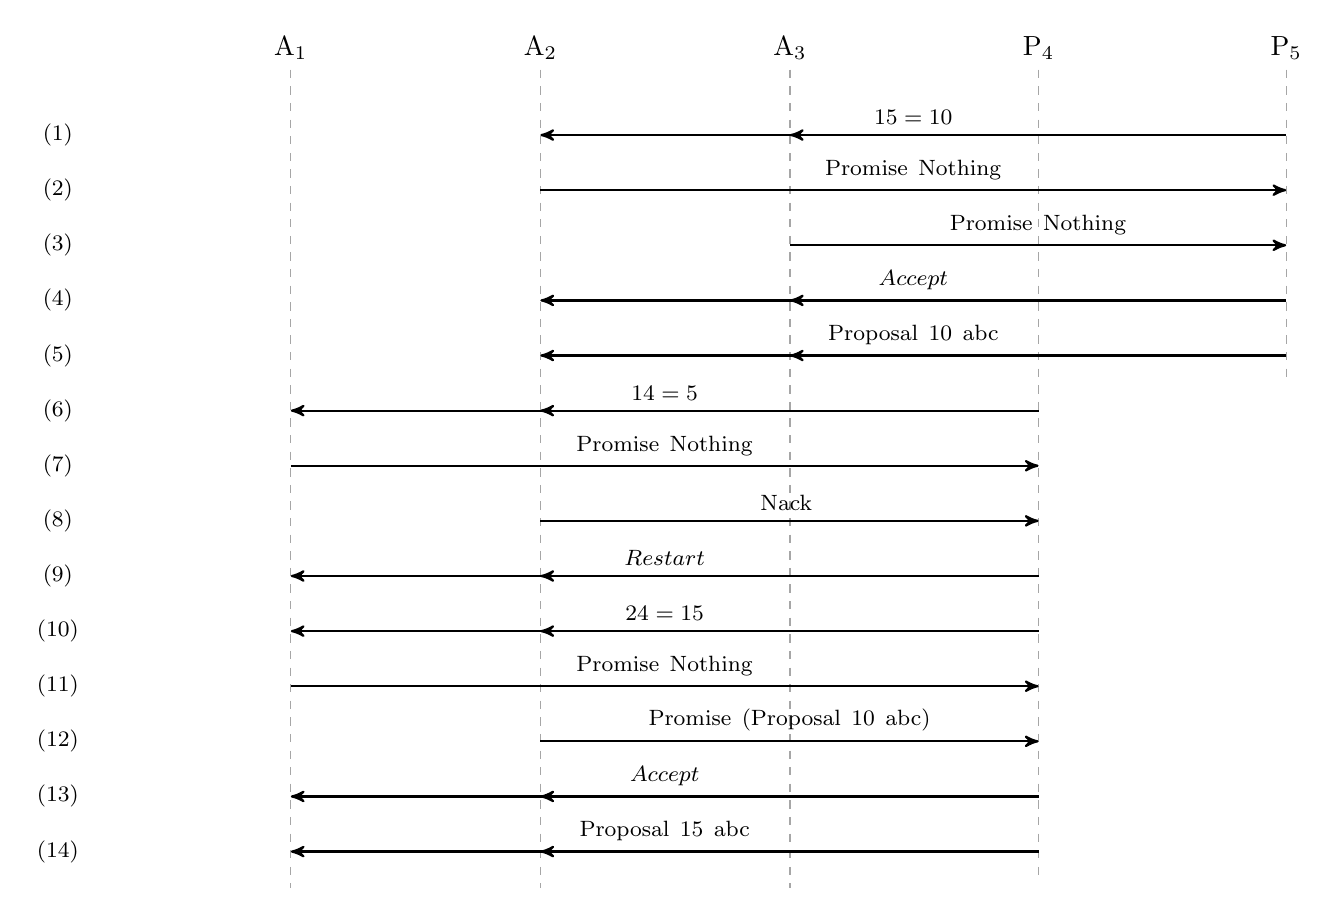
\begin{tikzpicture}[node distance=2.5cm, >=stealth', arrt/.style={above, font=\footnotesize}, arr/.style={->, thick}, lifeline/.style={dashed, black!35}]
    \def\InitialOffset{0.4}
    \def\StepSize{0.7}
    \newcommand{\Step}[1]{\InitialOffset + #1 * \StepSize}
    \def\MaxSteps{14}
    \def\FullHeight{\Step{\MaxSteps} + 0.66 * \StepSize}

    \node (a1) {$\Acceptor{1}$};
    \node[right = of a1] (a2) {$\Acceptor{2}$};
    \node[right = of a2] (a3) {$\Acceptor{3}$};
    \node[right = of a3] (p4) {$\Proposer{4}$};
    \node[right = of p4] (p5) {$\Proposer{5}$};
    \node[left = of a1] (notes) {};

    \draw[lifeline] (a1) -- ($(a1) - (0, \FullHeight)$);
    \draw[lifeline] (a2) -- ($(a2) - (0, \FullHeight)$);
    \draw[lifeline] (a3) -- ($(a3) - (0, \FullHeight)$);
    \draw[lifeline] (p4) -- ($(p4) - (0, \Step{14.5})$);
    \draw[lifeline] (p5) -- ($(p5) - (0, \Step{5.5})$);
    
    \draw[arr] ($(p5) - (0, \Step{1})$) -- node[arrt] {$\proposalNumber{1}{5} = 10$} ($(a2) - (0, \Step{1})$);
    \draw[arr] ($(p5) - (0, \Step{1})$) -- ($(a3) - (0, \Step{1})$);

    \draw[arr] ($(a2) - (0, \Step{2})$) -- node[arrt] {$\Promise{\Nothing}$} ($(p5) - (0, \Step{2})$);

    \draw[arr] ($(a3) - (0, \Step{3})$) -- node[arrt] {$\Promise{\Nothing}$} ($(p5) - (0, \Step{3})$);

    \draw[arr] ($(p5) - (0, \Step{4})$) -- node[arrt] {$\Accept$} ($(a2) - (0, \Step{4})$);
    \draw[arr] ($(p5) - (0, \Step{4})$) -- ($(a3) - (0, \Step{4})$);

    \draw[arr] ($(p5) - (0, \Step{5})$) -- node[arrt] {$\ProposalC{10}{\ABC}$} ($(a2) - (0, \Step{5})$);
    \draw[arr] ($(p5) - (0, \Step{5})$) -- ($(a3) - (0, \Step{5})$);

    \draw[arr] ($(p4) - (0, \Step{6})$) -- node[arrt] {$\proposalNumber{1}{4} = 5$} ($(a1) - (0, \Step{6})$);
    \draw[arr] ($(p4) - (0, \Step{6})$) -- ($(a2) - (0, \Step{6})$);

    \draw[arr] ($(a1) - (0, \Step{7})$) -- node[arrt] {$\Promise{\Nothing}$} ($(p4) - (0, \Step{7})$);

    \draw[arr] ($(a2) - (0, \Step{8})$) -- node[arrt] {$\Nack$} ($(p4) - (0, \Step{8})$);

    \draw[arr] ($(p4) - (0, \Step{9})$) -- node[arrt] {$\Restart$} ($(a1) - (0, \Step{9})$);
    \draw[arr] ($(p4) - (0, \Step{9})$) -- ($(a2) - (0, \Step{9})$);

    \draw[arr] ($(p4) - (0, \Step{10})$) -- node[arrt] {$\proposalNumber{2}{4} = 15$} ($(a1) - (0, \Step{10})$);
    \draw[arr] ($(p4) - (0, \Step{10})$) -- ($(a2) - (0, \Step{10})$);

    \draw[arr] ($(a1) - (0, \Step{11})$) -- node[arrt] {$\Promise{\Nothing}$} ($(p4) - (0, \Step{11})$);
    
    \draw[arr] ($(a2) - (0, \Step{12})$) -- node[arrt] {$\Promise{\Paren{\ProposalC{10}{\ABC}}}$} ($(p4) - (0, \Step{12})$);

    \draw[arr] ($(p4) - (0, \Step{13})$) -- node[arrt] {$\Accept$} ($(a1) - (0, \Step{13})$);
    \draw[arr] ($(p4) - (0, \Step{13})$) -- ($(a2) - (0, \Step{13})$);

    \draw[arr] ($(p4) - (0, \Step{14})$) -- node[arrt] {$\ProposalC{15}{\ABC}$} ($(a1) - (0, \Step{14})$);
    \draw[arr] ($(p4) - (0, \Step{14})$) -- ($(a2) - (0, \Step{14})$);

    \foreach \r in {1,...,\MaxSteps} {
        \node[font=\footnotesize] at ($(notes) - (0, \Step{\r})$) {$(\r)$};
    }
\end{tikzpicture}
\end{center}
\caption{Example scenario with $3$ acceptors and $2$ proposers.}
\label{fig:scenario}
\end{figure}

\subsection{Scenario}
Figure \ref{fig:scenario} provides an overview where $\Acceptor{1}$, $\Acceptor{2}$, and $\Acceptor{3}$ are the acceptors and $\Proposer{4}$ and $\Proposer{5}$ are the proposers.
$\Proposer{5}$ is elected to be the leader.
In steps $\Paren{1}$ to $\Paren{5}$, $\Proposer{5}$ completes the Paxos algorithm with $\Acceptor{2}$ and $\Acceptor{3}$ and terminates.

At this point $\Acceptor{2}$ has promised not to accept any proposal numbered less than $10$ and has accepted the value $\ABC$.
So, when $\Proposer{4}$ tries to use $5$ as its proposal number $\Paren{6}$, it receives $\Nack$ from $\Acceptor{2}$ $\Paren{8}$ and has to restart the algorithm $\Paren{9}$.

$\Proposer{4}$ then runs through the Paxos algorithm with $\Acceptor{1}$ and $\Acceptor{2}$ starting with a new prepare request $\Paren{10}$ with a higher proposal number.
In step $\Paren{12}$ $\Proposer{4}$ learns that value $\ABC$ with proposal number $10$ has already been accepted by $\Acceptor{2}$.
Later, in step $\Paren{14}$, $\Proposer{4}$ issues a proposal with the value of the highest-numbered proposal that it receives as a response to its prepare request.
In this case there is only one such proposal, which is $\ProposalC{10}{\ABC}$.

In the end all $3$ acceptors have accepted the value $\ABC$.
$\Acceptor{1}$ and $\Acceptor{2}$ have accepted $\ProposalC{15}{\ABC}$ and $\Acceptor{3}$ has accepted $\ProposalC{10}{\ABC}$.

\subsection{Formulae}
We set $\AcceptorCount = 3$, $\ProposerCount = 2$,
$\Value=\Curly{\ABC, \operatorname{def}, \ldots, \operatorname{vwx}, \operatorname{yz}}$.
$\AQ_4 = \genAq{4}{3}{2} = \Bracket{1,2}$ will be the quorum for $\Proposer{4}$ and $\AQ_5 = \genAq{5}{3}{2} = \Bracket{2,3}$ will be the quorum for $\Proposer{5}$.

Let $\NumberRegister_1$, $\NumberRegister_2$, $\NumberRegister_3$, $\NumberRegister_4$, $\NumberRegister_5$, $\ProposalRegister_1$, $\ProposalRegister_2$, and $\ProposalRegister_3$ be registers.
$\NumberRegister_1$, $\NumberRegister_2$, and $\NumberRegister_3$ hold a value of type $\Maybe{\mathbb{N}}$.
$\NumberRegister_4$ and $\NumberRegister_5$ hold a value of type $\mathbb{N}$.
$\ProposalRegister_1$, $\ProposalRegister_2$, and $\ProposalRegister_3$ hold a value of type $\Maybe{\Paren{\Proposal{\Value}}}$.
$\NumberRegister_{\ProcessIndexJ}$ and $\ProposalRegister_{\ProcessIndexJ}$ correspond to acceptor $\Acceptor{\ProcessIndexJ}$ for $\ProcessIndexJ \in \Curly{1, 2, 3}$.
$\NumberRegister_{\ProcessIndexK}$ corresponds to proposer $\Proposer{\ProcessIndexK}$ for $\ProcessIndexK \in \Curly{4, 5}$.
We set the following initial values.

\RegisterContent{$\Nothing$}{$\Nothing$}{$\Nothing$}{$0$}{$0$}{$\Nothing$}{$\Nothing$}{$\Nothing$}

\subsubsection{System Initialization}
\begin{align*}
\Sys{3}{2} =
&
    \SessionRequest{\OuterSharedPoint}{2}{\OuterSessionChannel}.
    \PpInit{5, 3, \Curly{1, 2}, 3, \NumberRegister_5, \EmptyList}
    \\
&\Or
    \SessionAccept{\OuterSharedPoint}{1}{\OuterSessionChannel}.
    \ParallelFor{3 < k < 5}
    \PpInit{\ProcessIndexK, 3, \Curly{1, 2}, 3, \NumberRegister_{\ProcessIndexK}, \EmptyList}
    \\
&\Or
    \ParallelFor{1 \le \ProcessIndexJ \le 3}
    \PaInit{\ProcessIndexJ, 3, 2, \NumberRegister_{\ProcessIndexJ}, \ProposalRegister_{\ProcessIndexJ}}
\end{align*}

After inserting $\AcceptorCount$ and $\ProposerCount$ and applying $\RInit$ once for shared channel $\OuterSharedPoint$ we have:

\begin{align*}
\mapstostar& \Nu{\OuterSessionChannel}\big (\\
&\SessionRequest{\SharedPoint{5}}{3}{\ChannelR}.\PpOne{\ChannelR, 5, 3, \Curly{1, 2}, 3, \NumberRegister_5, \EmptyList} \comment{= \Proposer{5}}\\
&\Or \SessionRequest{\SharedPoint{4}}{3}{\ChannelS}.\PpOne{\ChannelS, 4, 3, \Curly{1, 2}, 3, \NumberRegister_4, \EmptyList} \comment{= \Proposer{4}}\\
&\Or \Paren{
    \If 1 \notin \Curly{1, 2}
    \;\Then \End
    \;\Else \SessionAccept{\SharedPoint{4}}{1}{\ChannelS}\ldots
    \Or
    \If 1 \notin \Curly{2, 3}
    \;\Then \End
    \Else \ldots
} \comment{= \Acceptor{1}}\\
&\Or \Paren{
    \If 2 \notin \Curly{1, 2}
    \;\Then \End
    \;\Else \SessionAccept{\SharedPoint{4}}{2}{\ChannelS}\ldots
    \Or
    \If 2 \notin \Curly{2, 3}
    \;\Then \End
    \;\Else \SessionAccept{\SharedPoint{5}}{1}{\ChannelR}\ldots
} \comment{= \Acceptor{2}}\\
&\Or \Paren{
    \If 3 \notin \Curly{1, 2}
    \;\Then \End
    \;\Else \ldots
    \Or
    \If 3 \notin \Curly{2, 3}
    \;\Then \End
    \;\Else \SessionAccept{\SharedPoint{5}}{2}{\ChannelR}\ldots
} \comment{= \Acceptor{3}}\\
&\Or \OuterSessionQueues
\big )
\end{align*}

We apply $\RIfT$ to the left subprocess of $\Acceptor{3}$ and the right subprocess of $\Acceptor{1}$ and terminate them.
All other acceptor subprocesses advance by applying $\RIfF$.
Note that each process is shortened to only show the next few steps instead of the entire process.

\begin{align*}
\mapstostar& \NuChannels \big (\\
&\SessionRequest{\SharedPoint{5}}{3}{\ChannelR}.\PpOne{\ChannelR, 5, 3, \Curly{1, 2}, 3, \NumberRegister_5, \EmptyList} \comment{= \Proposer{5}}\\
&\Or \SessionRequest{\SharedPoint{4}}{3}{\ChannelS}.\PpOne{\ChannelS, 4, 3, \Curly{1, 2}, 3, \NumberRegister_4, \EmptyList} \comment{= \Proposer{4}}\\
&\Or \SessionAccept{\SharedPoint{4}}{1}{\ChannelS} . \PaOne{\ChannelS, 1, 3, \NumberRegister_1, \ProposalRegister_1} \comment{= \Acceptor{1}}\\
&\Or \Paren{
    \SessionAccept{\SharedPoint{4}}{2}{\ChannelS} . \PaOne{\ChannelS, 2, 3, \NumberRegister_2, \ProposalRegister_2}
    \Or
    \SessionAccept{\SharedPoint{5}}{1}{\ChannelR} . \PaOne{\ChannelR, 1, 3, \NumberRegister_2, \ProposalRegister_2}
} \comment{= \Acceptor{2}}\\
&\Or \SessionAccept{\SharedPoint{5}}{2}{\ChannelR} . \PaOne{\ChannelR, 2, 3, \NumberRegister_3, \ProposalRegister_3} \comment{= \Acceptor{3}}\\
&\Or \OuterSessionQueues
\big )
\end{align*}

We apply $\RInit$ for each shared channel $\SharedPoint{4}$ and $\SharedPoint{5}$ and unfold the calls to $\PpOne{\ChannelS, \ProcessIndexK, \ProposerRole, \QRoles, \AcceptorCount, \NumberRegister, \VectorV}$ and $\PaOne{\ChannelS, \AcceptorRole, \ProposerRole, \NumberRegister, \ProposalRegister}$ to obtain:

\begin{align*}
\mapstostar& \NuChannels\big (\\
&\Mu{\RecursionVariable} \update{\NumberRegister_5}{0 + 1} . \DotForall{\AcceptorRole\in \Curly{1, 2}}{\SendUnreliableP{\ChannelR}{3}{\AcceptorRole}{\LOneA}{\proposalNumber{\NumberRegister_5}{5}}}\ldots \comment{= \Proposer{5}}\\
&\Or \Mu{\RecursionVariable} \update{\NumberRegister_4}{0 + 1} . \DotForall{\AcceptorRole\in \Curly{1, 2}}{\SendUnreliableP{\ChannelS}{3}{\AcceptorRole}{\LOneA}{\proposalNumber{\NumberRegister_4}{4}}}\ldots \comment{= \Proposer{4}}\\
&\Or
    \Mu{\RecursionVariable}
    \ReceiveUnreliableP{\ChannelS}{1}{3}{\LOneA}{\bot}{n'}.
    \If \ldots \comment{= \Acceptor{1}}\\
&\Or \Paren{
    \Mu{\RecursionVariable} \ReceiveUnreliableP{\ChannelS}{2}{3}{\LOneA}{\bot}{n'}.\If \ldots
    \Or \Mu{\RecursionVariable} \ReceiveUnreliableP{\ChannelR}{1}{3}{\LOneA}{\bot}{n'}.\If \ldots
} \comment{= \Acceptor{2}}\\
&\Or \Mu{\RecursionVariable} \ReceiveUnreliableP{\ChannelR}{2}{3}{\LOneA}{\bot}{n'}.\If \ldots \comment{= \Acceptor{3}}\\
&\Or \InnerSessionQueues{\ChannelS}
\Or \InnerSessionQueues{\ChannelR}
\Or \OuterSessionQueues
\big )
\end{align*}

\subsubsection{The Happy Path}
We apply $\RRec$ to every process and $\RSideEffect$ to both proposers.
Now, the first inter-process communication can take place.
In this case $\Proposer{5}$ communicates with $\Acceptor{2}$ and $\Acceptor{3}$.
We apply $\RUsend$ and $\RUget$ twice to send $\proposalNumber{1}{5} = 10$ to $\Acceptor{2}$ and $\Acceptor{3}$.
% corresponds to (1)

\begin{align*}
&\mapstostar
\NuChannels \big (\\
&\ReceiveUnreliableP{\ChannelR}{3}{1}{\LOneB}{\bot}{v_1}.\ReceiveUnreliableP{\ChannelR}{3}{2}{\LOneB}{\bot}{v_2}\ldots \comment{= \Proposer{5}}\\
&\Or  \SendUnreliableP{\ChannelS}{3}{1}{\LOneA}{\proposalNumber{1}{4}}.\SendUnreliableP{\ChannelS}{3}{2}{\LOneA}{\proposalNumber{1}{4}}\ldots \comment{= \Proposer{4}}\\
&\Or  \ReceiveUnreliableP{\ChannelS}{1}{3}{\LOneA}{\bot}{n'}.\If \ldots \comment{=\Acceptor{1}}\\
&\Or
    \Paren{
        \ReceiveUnreliableP{\ChannelS}{2}{3}{\LOneA}{\bot}{n'}.\If \ldots
        \Or
            \If 10 = \bot
            \;\Then \ldots
            \;\Else \Paren{
                \If \greaterThan{10}{\NumberRegister_2} \ldots
                }
    } \comment{=\Acceptor{2}}\\
&\Or \If 10 = \bot
        \;\Then \ldots
        \;\Else \Paren{
            \If \greaterThan{n'}{\NumberRegister_3}
            \;\Then \update{\NumberRegister_3}{n'}\ldots
            \;\Else \ldots
        } \comment{=\Acceptor{3}}\\
&\Or \InnerSessionQueues{\ChannelS}
\Or \InnerSessionQueues{\ChannelR}
\Or \OuterSessionQueues
\big )
\end{align*}

Since $10 \neq \bot$ both $\Acceptor{2}$ and $\Acceptor{3}$ move into their respective $\ElseName$ branches by applying $\RIfF$.

\begin{align*}
\mapstostar& \NuChannels \big (\\
&\ReceiveUnreliableP{\ChannelR}{3}{1}{\LOneB}{\bot}{v_1}.\ReceiveUnreliableP{\ChannelR}{3}{2}{\LOneB}{\bot}{v_2}\ldots \comment{= \Proposer{5}}\\
&\Or \SendUnreliableP{\ChannelS}{3}{1}{\LOneA}{\proposalNumber{1}{4}}.\SendUnreliableP{\ChannelS}{3}{2}{\LOneA}{\proposalNumber{1}{4}}\ldots \comment{= \Proposer{4}}\\
&\Or \ReceiveUnreliableP{\ChannelS}{1}{3}{\LOneA}{\bot}{n'}.\If \ldots \comment{=\Acceptor{1}}\\
&\Or \Paren{
    \ReceiveUnreliableP{\ChannelS}{2}{3}{\LOneA}{\bot}{n'}.\If \ldots
    \Or
    \If \greaterThan{10}{\Nothing}
    \;\Then \ldots
    \;\Else \ldots
} \comment{=\Acceptor{2}}\\
&\Or
    \If \greaterThan{10}{\Nothing}
    \;\Then
        \update{\NumberRegister_3}{\Just{n'}}.
        \SendUnreliableP{\ChannelR}{2}{3}{\LOneB}{\Promise{\ProposalRegister_3}}\ldots
    \;\Else \ldots
    \comment{=\Acceptor{3}}\\
&\Or \InnerSessionQueues{\ChannelS}
\Or \InnerSessionQueues{\ChannelR}
\Or \OuterSessionQueues
\big )
\end{align*}

Because $\greaterThan{10}{\Nothing}$ returns $\True$, $\Acceptor{2}$ and $\Acceptor{3}$ move into their respective $\ThenName$ branches by applying $\RIfT$.
After executing $\update{\NumberRegister_2}{\Just{10}}$ and $\update{\NumberRegister_3}{\Just{10}}$ with $\RSideEffect$, $\Acceptor{2}$ and $\Acceptor{3}$ are ready to send their responses to $\Proposer{5}$.

% A1: n=Nothing, pr=Nothing
% A2: n=10, pr=Nothing
% A3: n=10, pr=Nothing
%  P^A_2 (s, a, p, n, pr)
\begin{align*}
\mapstostar& \NuChannels \big (\\
&
    \ReceiveUnreliableP{\ChannelR}{3}{1}{\LOneB}{\bot}{v_1}.
    \ReceiveUnreliableP{\ChannelR}{3}{2}{\LOneB}{\bot}{v_2}.
    \If \anyNack{\VectorV} \tOr \promiseCount{\VectorV} < 2\ldots
    \comment{= \Proposer{5}}\\
&\Or \SendUnreliableP{\ChannelS}{3}{1}{\LOneA}{\proposalNumber{1}{4}}.\SendUnreliableP{\ChannelS}{3}{2}{\LOneA}{\proposalNumber{1}{4}}\ldots \comment{= \Proposer{4}}\\
&\Or \ReceiveUnreliableP{\ChannelS}{1}{3}{\LOneA}{\bot}{n'}.\If \ldots \comment{= \Acceptor{1}}\\
&\Or \Paren{
    \ReceiveUnreliableP{\ChannelS}{2}{3}{\LOneA}{\bot}{n'}.\If \ldots
    \Or \SendUnreliableP{\ChannelR}{1}{3}{\LOneB}{\Promise{\Nothing}}.
        \PaTwo{\ChannelR, 1, 3, \NumberRegister_2, \ProposalRegister_2}
} \comment{= \Acceptor{2}}\\
&\Or
    \SendUnreliableP{\ChannelR}{2}{3}{\LOneB}{\Promise{\Nothing}}.
    \PaTwo{\ChannelR, 2, 3, \NumberRegister_3, \ProposalRegister_3}
    \comment{= \Acceptor{3}}\\
&\Or \InnerSessionQueues{\ChannelS}
\Or \InnerSessionQueues{\ChannelR}
\Or \OuterSessionQueues
\big )
\end{align*}

We apply $\RUsend$ and $\RUget$ twice to do just that.
$\Acceptor{3}$ and one subprocess of $\Acceptor{2}$ move into $\PaTwo{\SessionChannel, \AcceptorRole, \ProposerRole, \NumberRegister, \ProposalRegister}$.

$\Proposer{5}$ has $\VectorV = \Bracket{\Promise{\Nothing}, \Promise{\Nothing}}$.
$\anyNack{\VectorV}$ returns $\False$ and $\promiseCount{\VectorV}$ returns $2$.
Thus, $\anyNack{\VectorV} \tOr \promiseCount{\VectorV} < 2$ evaluates to $\False$.
By applying $\RIfF$ $\Proposer{5}$ advances to its $\ElseName$ branch.
% corresponds to (2) - (3)

\begin{align*}
\mapstostar& \NuChannels \big (\\
&
    \SendWeaklyP{\ChannelR}{3}{\Curly{1, 2}}{\Accept}.
    \SendUnreliableP{\ChannelR}{3}{1}{\LTwoA}{\ProposalC{10}{\ABC}}\ldots
    \comment{= \Proposer{5}}\\
&\Or \SendUnreliableP{\ChannelS}{3}{1}{\LOneA}{\proposalNumber{1}{4}}.\SendUnreliableP{\ChannelS}{3}{2}{\LOneA}{\proposalNumber{1}{4}}\ldots \comment{= \Proposer{4}}\\
&\Or \ReceiveUnreliableP{\ChannelS}{1}{3}{\LOneA}{\bot}{n'}.\If \ldots \comment{= \Acceptor{1}}\\
&\Or \Paren{
    \ReceiveUnreliableP{\ChannelS}{2}{3}{\LOneA}{\bot}{n'}.\If \ldots
    \Or \ReceiveWeaklyP{\ChannelR}{1}{3}{\BeginPaCont}
} \comment{= \Acceptor{2}}\\
&\Or
    \ReceiveWeaklyP{\ChannelR}{2}{3}{
        \Accept. \PaThree{\ChannelR, 2, 3, \NumberRegister_3, \ProposalRegister_3} \oplus \Restart. \RecursionVariable \oplus \Abort . \End
    }
    \comment{= \Acceptor{3}}\\
&\Or \InnerSessionQueues{\ChannelS}
\Or \InnerSessionQueues{\ChannelR}
\Or \OuterSessionQueues
\big )
\end{align*}

$\Proposer{5}$ broadcasts its decision $\Accept$ to $\Acceptor{2}$ and $\Acceptor{3}$.
By applying $\RWsel$ once, $\RWbran$ twice we obtain:
% corresponds to (4)

\begin{align*}
\mapstostar& \NuChannels \big (\\
&
    \SendUnreliableP{\ChannelR}{3}{1}{\LTwoA}{\ProposalC{10}{\ABC}}.
    \SendUnreliableP{\ChannelR}{3}{2}{\LTwoA}{\ProposalC{10}{\ABC}}.
    \End
    \comment{= \Proposer{5}}\\
&\Or
    \SendUnreliableP{\ChannelS}{3}{1}{\LOneA}{\proposalNumber{1}{4}}.
    \SendUnreliableP{\ChannelS}{3}{2}{\LOneA}{\proposalNumber{1}{4}}\ldots
    \comment{= \Proposer{4}}\\
&\Or \ReceiveUnreliableP{\ChannelS}{1}{3}{\LOneA}{\bot}{n'}.\If \ldots \comment{= \Acceptor{1}}\\
&\Or \Paren{
    \ReceiveUnreliableP{\ChannelS}{2}{3}{\LOneA}{\bot}{n'}.\If \ldots
    \Or \ReceiveUnreliableP{\ChannelR}{1}{3}{\LTwoA}{\bot}{pr'}.\If \ldots
} \comment{= \Acceptor{2}}\\
&\Or
    \ReceiveUnreliableP{\ChannelR}{2}{3}{\LTwoA}{\bot}{pr'}.
    \If pr' = \bot
    \;\Then \End
    \;\Else \Paren{\If \ldots}
    \comment{= \Acceptor{3}}\\
&\Or \InnerSessionQueues{\ChannelS}
\Or \InnerSessionQueues{\ChannelR}
\Or \OuterSessionQueues
\big )
\end{align*}

Now $\Proposer{5}$ can send its proposal to $\Acceptor{2}$ and $\Acceptor{3}$ and terminate.
To do so we apply $\RUsend$ and $\RUget$ twice.

\begin{align*}
&\mapstostar\NuChannels\big (\\
&\Or
\SendUnreliableP{\ChannelS}{3}{1}{\LOneA}{\proposalNumber{1}{4}}.
\SendUnreliableP{\ChannelS}{3}{2}{\LOneA}{\proposalNumber{1}{4}}\ldots
\comment{= \Proposer{4}}\\
&\Or \ReceiveUnreliableP{\ChannelS}{1}{3}{\LOneA}{\bot}{n'}.\If \ldots \comment{= \Acceptor{1}}\\
&\Or
    \Paren{
        \ReceiveUnreliableP{\ChannelS}{2}{3}{\LOneA}{\bot}{n'}.\If \ldots
        \Or
        \If \Paren{\ProposalC{10}{\ABC}} = \bot
        \;\Then \End
        \;\Else \Paren{\If \ldots}
    } \comment{= \Acceptor{2}}\\
&\Or
    \If \Paren{\ProposalC{10}{\ABC}} = \bot
    \;\Then \End
    \;\Else \Paren{
        \If \greaterEqual{10}{\NumberRegister_3}
        \;\Then \update{\ProposalRegister_3}{\Just{pr'}}\ldots
        \;\Else \End
    }
    \comment{= \Acceptor{3}}\\
&\Or \InnerSessionQueues{\ChannelS}
\Or \InnerSessionQueues{\ChannelR}
\Or \OuterSessionQueues
\big )
\end{align*}

Because $\Paren{\ProposalC{10}{\ABC}} = \bot$ evaluates to $\False$ we can apply $\RIfF$ to $\Acceptor{2}$ and $\Acceptor{3}$.
Then, we can apply $\RIfT$ to $\Acceptor{2}$ and $\Acceptor{3}$ because $\greaterEqual{10}{\Just{10}}$ returns $\True$.

\begin{align*}
&\mapstostar\NuChannels\big (\\
&\Or
\SendUnreliableP{\ChannelS}{3}{1}{\LOneA}{\proposalNumber{1}{4}}.
\SendUnreliableP{\ChannelS}{3}{2}{\LOneA}{\proposalNumber{1}{4}}\ldots
\comment{= \Proposer{4}}\\
&\Or \ReceiveUnreliableP{\ChannelS}{1}{3}{\LOneA}{\bot}{n'}.\If \ldots \comment{= \Acceptor{1}}\\
&\Or
    \Paren{
        \ReceiveUnreliableP{\ChannelS}{2}{3}{\LOneA}{\bot}{n'}.\If \ldots
        \Or
            \update{\ProposalRegister_2}{\Just{\Paren{\ProposalC{10}{\ABC}}}}.
            \update{\NumberRegister_2}{\Just{10}}.
            \End
    } \comment{= \Acceptor{2}}\\
&\Or
    \update{\ProposalRegister_3}{\Just{\Paren{\ProposalC{10}{\ABC}}}}.
    \update{\NumberRegister_3}{\Just{10}}.
    \End
    \comment{= \Acceptor{3}}\\
&\Or \InnerSessionQueues{\ChannelS}
\Or \InnerSessionQueues{\ChannelR}
\Or \OuterSessionQueues
\big )
\end{align*}

$\Acceptor{2}$ and $\Acceptor{3}$ terminate after applying $\RSideEffect$ twice and updating their registers.
They have accepted the proposal.
$\Proposer{4}$ is the new leader.
% corresponds to (5)

\begin{align*}
&\mapstostar\NuChannels\big (\\
&\Or
\SendUnreliableP{\ChannelS}{3}{1}{\LOneA}{5}.
\SendUnreliableP{\ChannelS}{3}{2}{\LOneA}{5}\ldots
\comment{= \Proposer{4}}\\
&\Or
    \ReceiveUnreliableP{\ChannelS}{1}{3}{\LOneA}{\bot}{n'}.
    \If n' = \bot
    \;\Then \ldots
    \;\Else \Paren{
        \If \greaterThan{n'}{\NumberRegister_1}
        \ldots
    }
    \comment{= \Acceptor{1}}\\
&\Or
    \ReceiveUnreliableP{\ChannelS}{2}{3}{\LOneA}{\bot}{n'}.
    \If n' = \bot
    \;\Then \ldots
    \;\Else \Paren{
        \If \greaterThan{n'}{\NumberRegister_2}
        \ldots
    }
    \comment{= \Acceptor{2}}\\
&\Or \InnerSessionQueues{\ChannelS}
\Or \OuterSessionQueues
\big )
\end{align*}

At this point the registers hold the following values.

\RegisterContent{$\Nothing$}{$\Just{10}$}{$\Just{10}$}{$1$}{$1$}{$\Nothing$}{$\Just{\Paren{\ProposalC{10}{\ABC}}}$}{$\Just{\Paren{\ProposalC{10}{\ABC}}}$}

\subsubsection{Restarting The Algorithm}
Next, $\Proposer{4}$ sends prepare requests with a proposal number less than $10$, which $\Acceptor{2}$ rejects.
$\Proposer{4}$ then decides to restart the algorithm.
We apply $\RUsend$ and $\RUget$ twice.

\begin{align*}
&\mapstostar\NuChannels\big (\\
&\Or
    \ReceiveUnreliableP{\ChannelS}{3}{1}{\LOneB}{\bot}{v_1}.
    \ReceiveUnreliableP{\ChannelS}{3}{2}{\LOneB}{\bot}{v_2}.
    \ldots
    \comment{= \Proposer{4}}\\
&\Or
    \If 5 = \bot
    \;\Then \ldots
    \;\Else \Paren{
        \If \greaterThan{5}{\NumberRegister_1}
        \;\Then \update{\NumberRegister_1}{\Just{5}}\ldots
        \;\Else \ldots
    }
    \comment{= \Acceptor{1}}\\
&\Or
    \If 5 = \bot
    \;\Then \ldots
    \;\Else \Paren{
        \If \greaterThan{5}{\NumberRegister_2}
        \;\Then \ldots
        \;\Else
            \SendUnreliableP{\ChannelS}{2}{3}{\LOneB}{\Nack}.
            \PaTwo{\ChannelS, 2, 3, \NumberRegister_2, \ProposalRegister_2}
    }
    \comment{= \Acceptor{2}}\\
&\Or \InnerSessionQueues{\ChannelS}
\Or \OuterSessionQueues
\big )
\end{align*}

Because $5 = \bot$ evaluates to $\False$ we apply $\RIfF$ to $\Acceptor{1}$ and $\Acceptor{2}$.
We apply $\RIfF$ to $\Acceptor{2}$ again because $\greaterThan{5}{\Just{10}}$ returns $\False$.
$\greaterThan{5}{\Nothing}$ returns $\True$, so we advance $\Acceptor{1}$ to its $\ThenName$ branch by applying $\RIfT$.

\begin{align*}
&\mapstostar\NuChannels\big (\\
&\Or
    \ReceiveUnreliableP{\ChannelS}{3}{1}{\LOneB}{\bot}{v_1}.
    \ReceiveUnreliableP{\ChannelS}{3}{2}{\LOneB}{\bot}{v_2}.
    \ldots
    \comment{= \Proposer{4}}\\
&\Or
    \update{\NumberRegister_1}{\Just{5}}.
    \SendUnreliableP{\ChannelS}{1}{3}{\LOneB}{\Promise{\Nothing}}.
    \PaTwo{\ChannelS, 1, 3, \NumberRegister_1, \ProposalRegister_1}
    \comment{= \Acceptor{1}}\\
&\Or
    \SendUnreliableP{\ChannelS}{2}{3}{\LOneB}{\Nack}.
    \PaTwo{\ChannelS, 2, 3, \NumberRegister_2, \ProposalRegister_2}
    \comment{= \Acceptor{2}}\\
&\Or \InnerSessionQueues{\ChannelS}
\Or \OuterSessionQueues
\big )
\end{align*}

We apply $\RSideEffect$ to $\Acceptor{1}$ to update its register $\NumberRegister_1$.
Applying $\RUsend$ and $\RUget$ twice then yields:

\begin{align*}
&\mapstostar\NuChannels\big (\\
&\Or
    \If \anyNack{\VectorV} \tOr \promiseCount{\VectorV} < 2
    \;\Then \SendWeaklyP{\ChannelS}{3}{\Curly{1, 2}}{\Restart}. \RecursionVariable
    \;\Else \ldots
    \comment{= \Proposer{4}}\\
&\Or
    \ReceiveWeaklyP{\ChannelS}{1}{3}{
        \Accept. \PaThree{\ChannelS, 1, 3, \NumberRegister_1, \ProposalRegister_1} \oplus \Restart. \RecursionVariable \oplus \Abort . \End
    }
    \comment{= \Acceptor{1}}\\
&\Or
    \ReceiveWeaklyP{\ChannelS}{2}{3}{
        \Accept. \PaThree{\ChannelS, 2, 3, \NumberRegister_2, \ProposalRegister_2} \oplus \Restart. \RecursionVariable \oplus \Abort . \End
    }
    \comment{= \Acceptor{2}}\\
&\Or \InnerSessionQueues{\ChannelS}
\Or \OuterSessionQueues
\big )
\end{align*}

$\Proposer{4}$ has $\VectorV = \Bracket{\Promise{\Nothing}, \Nack}$.
$\anyNack{\VectorV}$ returns $\True$ and $\promiseCount{\VectorV}$ returns 1.
Thus, $\anyNack{\VectorV} \tOr \promiseCount{\VectorV} < 2$ evaluates to $\True$.
We apply $\RIfT$ to $\Proposer{4}$.

\begin{align*}
\mapstostar& \NuChannels \big (\\
&
    \SendWeaklyP{\ChannelS}{3}{\Curly{1,2}}{\Restart}.
    \Mu{\RecursionVariable}
    \update{\NumberRegister_4}{\NumberRegister_4 + 1}.
    \SendUnreliableP{\ChannelS}{3}{1}{\LOneA}{\proposalNumber{\NumberRegister_4}{4}}\ldots
    \comment{= \Proposer{4}}\\
&\Or
    \ReceiveWeaklyP{\ChannelS}{1}{3}{
        \Accept \ldots
        \oplus
            \Restart .
            \Mu{\RecursionVariable} \ReceiveUnreliableP{\ChannelS}{1}{3}{\LOneA}{\bot}{n'}\ldots
        \oplus \Abort . \End
    } \comment{= \Acceptor{1}}\\
&\Or
    \ReceiveWeaklyP{\ChannelS}{2}{3}{
        \Accept \ldots
        \oplus
            \Restart .
            \Mu{\RecursionVariable} \ReceiveUnreliableP{\ChannelS}{2}{3}{\LOneA}{\bot}{n'}\ldots
        \oplus \Abort . \End
    } \comment{= \Acceptor{2}}\\
&\Or \InnerSessionQueues{\ChannelS}
\Or \OuterSessionQueues
\big )
\end{align*}

$\Proposer{4}$ sends its decision to restart the algorithm to $\Acceptor{1}$ and $\Acceptor{2}$ by applying $\RWsel$ once and $\RWbran$ twice.

\begin{align*}
\mapstostar& \NuChannels \big (\\
&
    \Mu{\RecursionVariable}
    \update{\NumberRegister_4}{2}.
    \SendUnreliableP{\ChannelS}{3}{1}{\LOneA}{15}.
    \SendUnreliableP{\ChannelS}{3}{2}{\LOneA}{15}.
    \ReceiveUnreliableP{\ChannelS}{3}{1}{\LOneB}{\bot}{v_1}\ldots
    \comment{= \Proposer{4}}\\
&\Or
    \Mu{\RecursionVariable}
    \ReceiveUnreliableP{\ChannelS}{1}{3}{\LOneA}{\bot}{n'}.
    \If n' = \bot
    \;\Then \ldots
    \;\Else
        \Paren{
            \If \greaterThan{n'}{\NumberRegister_1}
            \ldots
        }
    \comment{= \Acceptor{1}}\\
&\Or
    \Mu{\RecursionVariable}
    \ReceiveUnreliableP{\ChannelS}{2}{3}{\LOneA}{\bot}{n'}.
    \If n' = \bot
    \;\Then \ldots
    \;\Else
        \Paren{
            \If \greaterThan{n'}{\NumberRegister_2}
            \ldots
        }
    \comment{= \Acceptor{2}}\\
&\Or \InnerSessionQueues{\ChannelS}
\Or \OuterSessionQueues
\big )
\end{align*}

At this point the registers hold the following values.

\RegisterContent{$\Just{5}$}{$\Just{10}$}{$\Just{10}$}{$1$}{$1$}{$\Nothing$}{$\Just{\Paren{\ProposalC{10}{\ABC}}}$}{$\Just{\Paren{\ProposalC{10}{\ABC}}}$}

\subsubsection{The Happy Path, Again}

First, we apply $\RRec$ to each process and then $\RSideEffect$ to $\Proposer{4}$.

\begin{align*}
\mapstostar& \NuChannels \big (\\
&
    \SendUnreliableP{\ChannelS}{3}{1}{\LOneA}{15}.
    \SendUnreliableP{\ChannelS}{3}{2}{\LOneA}{15}.
    \ReceiveUnreliableP{\ChannelS}{3}{1}{\LOneB}{\bot}{v_1}\ldots
    \comment{= \Proposer{4}}\\
&\Or
    \ReceiveUnreliableP{\ChannelS}{1}{3}{\LOneA}{\bot}{n'}.
    \If n' = \bot
    \;\Then \ldots
    \;\Else \Paren{
            \If \greaterThan{n'}{\NumberRegister_1}
            \ldots
        }
    \comment{= \Acceptor{1}}\\
&\Or
    \ReceiveUnreliableP{\ChannelS}{2}{3}{\LOneA}{\bot}{n'}.
    \If n' = \bot
    \;\Then \ldots
    \;\Else \Paren{
        \If \greaterThan{n'}{\NumberRegister_2}
        \ldots
    }
    \comment{= \Acceptor{2}}\\
&\Or \InnerSessionQueues{\ChannelS}
\Or \OuterSessionQueues
\big )
\end{align*}

This time $\Proposer{4}$ uses a high enough proposal number so that $\Acceptor{1}$ and $\Acceptor{2}$ both promise not to accept any proposal numbered less than that.
$15 = \bot$ evaluates to $\False$ and $\greaterThan{15}{\Just{10}}$ and $\greaterThan{15}{\Just{5}}$ return $\True$.
By applying $\RUsend$ twice in the remaining proposer and $\RUget$, $\RIfF$, and $\RIfT$ in the remaining acceptors we arrive at:

% A1: n=15, pr=Nothing
% A2: n=15, pr=Proposal 10 abc
% A3: n=10, pr=Proposal 10 abc
\begin{align*}
\mapstostar& \NuChannels \big (\\
&
    \ReceiveUnreliableP{\ChannelS}{3}{1}{\LOneB}{\bot}{v_1}.
    \ReceiveUnreliableP{\ChannelS}{3}{2}{\LOneB}{\bot}{v_2}.
    \If \ldots
    \comment{= \Proposer{4}}\\
&\Or
    \update{\NumberRegister_1}{\Just{15}}.
    \SendUnreliableP{\ChannelS}{1}{3}{\LOneB}{\Promise{\Nothing}}.
    \PaTwo{\ChannelS, 1, 3, \NumberRegister_1, \ProposalRegister_1}
    \comment{= \Acceptor{1}}\\
&\Or
    \update{\NumberRegister_2}{\Just{15}}.
    \SendUnreliableP{\ChannelS}{2}{3}{\LOneB}{\Promise{\Paren{\ProposalC{10}{abc}}}}.
    \PaTwo{\ChannelS, 2, 3, \NumberRegister_2, \ProposalRegister_2} \comment{= \Acceptor{2}}\\
&\Or \InnerSessionQueues{\ChannelS}
\Or \OuterSessionQueues
\big )
\end{align*}

$\Acceptor{1}$ and $\Acceptor{2}$ update their respective registers $\NumberRegister$ to $\Just{15}$ by applying $\RSideEffect$.
Because $\Acceptor{2}$ has already accepted a proposal, it responds to $\Proposer{4}$'s prepare request with that proposal.
Twice more we apply $\RUsend$ and $\RUget$ to obtain:

% A1: n=15, pr=Nothing
% A2: n=15, pr=Proposal 10 abc
% A3: n=10, pr=Proposal 10 abc
\begin{align*}
\mapstostar& \NuChannels \big (\\
&
    \If \anyNack{\VectorV} \tOr \promiseCount{\VectorV} < 2
    \;\Then \ldots
    \;\Else
        \SendWeaklyP{\ChannelS}{3}{\Curly{1,2}}{\Accept}
        \ldots
    \comment{= \Proposer{4}}\\
&\Or
    \ReceiveWeaklyP{\ChannelS}{1}{3}{
        \Accept . \PaThree{\ChannelS, 1, 3 \NumberRegister_1, \ProposalRegister_1}
        \oplus \Restart. \RecursionVariable
        \oplus \Abort . \End
    }
    \comment{= \Acceptor{1}}\\
&\Or
    \ReceiveWeaklyP{\ChannelS}{2}{3}{
        \Accept . \PaThree{\ChannelS, 2, 3, \NumberRegister_2, \ProposalRegister_2}
        \oplus \Restart. \RecursionVariable
        \oplus \Abort . \End
    }
    \comment{= \Acceptor{2}}\\
&\Or \InnerSessionQueues{\ChannelS}
\Or \OuterSessionQueues
\big )
\end{align*}

$\Proposer{4}$ has $\VectorV = \Bracket{\Promise{\Nothing}, \Promise{\Paren{\Just{\Paren{\ProposalC{10}{\ABC}}}}}}$.
$\anyNack{\VectorV} \tOr \promiseCount{\VectorV} < 2$ evaluates to $\False$ and we can apply $\RIfF$.

\begin{align*}
\mapstostar& \NuChannels \big (\\
&
    \SendWeaklyP{\ChannelS}{3}{\Curly{1,2}}{\Accept}.
    \SendUnreliableP{\ChannelS}{3}{1}{\LTwoA}{\ProposalC{15}{\ABC}}.
    \SendUnreliableP{\ChannelS}{3}{2}{\LTwoA}{\ProposalC{15}{\ABC}}.
    \End
    \comment{= \Proposer{4}}\\
&\Or
    \ReceiveWeaklyP{\ChannelS}{1}{3}{
        \Accept . \PaThree{\ChannelS, 1, 3 \NumberRegister_1, \ProposalRegister_1}
        \oplus \Restart. \RecursionVariable
        \oplus \Abort . \End
    }
    \comment{= \Acceptor{1}}\\
&\Or
    \ReceiveWeaklyP{\ChannelS}{2}{3}{
        \Accept . \PaThree{\ChannelS, 2, 3, \NumberRegister_2, \ProposalRegister_2}
        \oplus \Restart. \RecursionVariable
        \oplus \Abort . \End
    }
    \comment{= \Acceptor{2}}\\
&\Or \InnerSessionQueues{\ChannelS}
\Or \OuterSessionQueues
\big )
\end{align*}

$\Proposer{4}$ has received enough promises to send its own proposal.
The value for that proposal is $\ABC$ because that is the value of the highest-numbered proposal $\Proposer{4}$ received as a response to its prepare request.
First, we apply $\RWsel$ and $\RWbran$.

% A1: n=15, pr=Nothing
% A2: n=15, pr=Proposal 10 abc
% A3: n=10, pr=Proposal 10 abc
\begin{align*}
\mapstostar& \NuChannels \big (\\
&
    \SendUnreliableP{\ChannelS}{3}{1}{\LTwoA}{\ProposalC{15}{\ABC}}.
    \SendUnreliableP{\ChannelS}{3}{2}{\LTwoA}{\ProposalC{15}{\ABC}}.
    \End
    \comment{= \Proposer{4}}\\
&\Or
    \ReceiveUnreliableP{\ChannelS}{1}{3}{\LTwoA}{\bot}{pr'}.
    \If pr' = \bot
    \;\Then \End
    \;\Else \Paren{
        \If \greaterEqual{\nFromProposal{pr'}}{\NumberRegister_1}
        \ldots
    }
    \comment{= \Acceptor{1}}\\
&\Or
    \ReceiveUnreliableP{\ChannelS}{2}{3}{\LTwoA}{\bot}{pr'}.
    \If pr' = \bot
    \;\Then \End
    \;\Else \Paren{
        \If \greaterEqual{\nFromProposal{pr'}}{\NumberRegister_2}
        \ldots
    }
    \comment{= \Acceptor{2}}\\
&\Or \InnerSessionQueues{\ChannelS}
\Or \OuterSessionQueues
\big )
\end{align*}

Then we apply $\RUsend$ and $\RUget$ to send the proposal from $\Proposer{4}$ to the acceptors.
$\Proposer{4}$ terminates.

\begin{align*}
\mapstostar& \NuChannels \big (\\
&
    \If \Paren{\ProposalC{15}{\ABC}} = \bot
    \;\Then \End
    \;\Else \Paren{
        \If \greaterEqual{15}{\NumberRegister_1}
        \;\Then \update{\ProposalRegister_1}{\Just{pr'}}\ldots
        \;\Else \End
    }
    \comment{= \Acceptor{1}}\\
&\Or
    \If \Paren{\ProposalC{15}{\ABC}} = \bot
    \;\Then \End
    \;\Else \Paren{
        \If \greaterEqual{15}{\NumberRegister_2}
        \;\Then \update{\ProposalRegister_2}{\Just{pr'}}\ldots
        \;\Else \End
    }
    \comment{= \Acceptor{2}}\\
&\Or \InnerSessionQueues{\ChannelS}
\Or \OuterSessionQueues
\big )
\end{align*}

$\Paren{\ProposalC{15}{\ABC}} = \bot$ evaluates to $\False$ and $\greaterEqual{15}{\Just{15}}$ returns $\True$.
So, we apply $\RIfF$ and then $\RIfT$ to the acceptors.

\begin{align*}
\mapstostar& \NuChannels \big (\\
&
    \update{\ProposalRegister_1}{\Just{pr'}}.
    \update{\NumberRegister_1}{\Just{\Paren{\nFromProposal{pr'}}}}.
    \End
    \comment{= \Acceptor{1}}\\
&\Or
    \update{\ProposalRegister_2}{\Just{pr'}}.
    \update{\NumberRegister_2}{\Just{\Paren{\nFromProposal{pr'}}}}.
    \End
    \comment{= \Acceptor{2}}\\
&\Or \InnerSessionQueues{\ChannelS}
\Or \OuterSessionQueues
\big )
\end{align*}

Finally, we apply $\RSideEffect$ twice to each acceptor.
With that, \Acceptor{1} and \Acceptor{2} have accepted \Proposer{4}'s proposal.

% A1: n=15, pr=Proposal 15 abc
% A2: n=15, pr=Proposal 15 abc
% A3: n=10, pr=Proposal 10 abc
\[\mapstostar \NuChannels \End\]

The final values the registers contain are as follows.

\RegisterContent{$\Just{15}$}{$\Just{15}$}{$\Just{10}$}{$2$}{$2$}{$\Just{\Paren{\ProposalC{15}{\ABC}}}$}{$\Just{\Paren{\ProposalC{15}{\ABC}}}$}{$\Just{\Paren{\ProposalC{10}{\ABC}}}$}

All acceptors have accepted the value $\ABC$.


% \IMRADlabel{results}
\chapter{Analysis}

\section{Local Types}
$\OuterGlobalTypeProjection{k} = \End$ for every $k$.

$\GlobalTypeProjection{i} = \LocalTypeProposer = \Mu{x}
\DotForall{j \in \AQ}{\SendUnreliableL{j}{\LOneA}{\mathbb{N}}} .
\DotForall{j \in \AQ}{\ReceiveUnreliableL{j}{\LOneB}{\Promise{\Value}}} .\\
\Indent{1}\SendWeaklyL{\AQ}{\Accept . \DotForall{j \in \AQ}{\SendUnreliableL{j}{\LTwoA}{\Proposal{\Value}}}.\End \oplus \Restart . x \oplus \Abort .\End}$

$\GlobalTypeProjection{j} = \LocalTypeAcceptor = \Mu{x}
\ReceiveUnreliableL{i}{\LOneA}{\mathbb{N}} .
\SendUnreliableL{i}{\LOneB}{\Promise{\Value}} .\\
\Indent{1}\ReceiveWeaklyL{i}{\Accept . \ReceiveUnreliableL{i}{\LTwoA}{\Proposal{\Value}}.\End \oplus \Restart . x \oplus \Abort .\End}$

\section{Type Check}
\subsection{System Initialization}
$\Gamma = \GEnvEntry{a}{\OuterGlobalType} \cdot \GEnvEntry{b_{ac+1}}{\GlobalType} \cdot \GEnvEntry{b_{ac+2}}{\GlobalType} \cdot \ldots \cdot \GEnvEntry{b_{ac+pc}}{\GlobalType}$.

\begin{prooftree}
\AxiomC{$\SysProof{1}$}
\UnaryInfC{$\Gamma\vdash \SessionRequest{a}{2}{t}\ldots \vartriangleright \emptyset$}

\AxiomC{$\SysProof{2}$}
\UnaryInfC{$\Gamma\vdash \SessionAccept{a}{1}{t} \ldots \vartriangleright \emptyset$}

\AxiomC{$\SysProof{3}$}
\UnaryInfC{$\Gamma\vdash \ParallelFor{1 \leq j \leq ac} \PaInitShort \vartriangleright \emptyset$}

\RightLabel{$\RPar$}
\BinaryInfC{$\Gamma\vdash \SessionAccept{a}{1}{t} \ldots \Or \ParallelFor{1 \leq j \leq ac} \PaInitShort \vartriangleright \emptyset$}

\RightLabel{$\RPar$}
\BinaryInfC{$\Gamma\vdash \SessionRequest{a}{2}{t}.\PpInitShort \Or \SessionAccept{a}{1}{t} \ldots \Or \ParallelFor{1 \leq j \leq ac} \PaInitShort \vartriangleright \emptyset$}
\end{prooftree}

\subsubsection{$\SysProof{1}$}
\begin{prooftree}
\AxiomC{$\ProposerProof{}$}
\UnaryInfC{$\Gamma\vdash \SessionRequest{b_{ac+pc}}{ac+1}{s}.\Pp{} \vartriangleright \SEnvEntry{t}{2}{\OuterGlobalTypeProjection{2}}$}

\LeftLabel{$\SysProof{1} =$}
\RightLabel{$\RRec$}
\UnaryInfC{$\Gamma\vdash \SessionRequest{a}{2}{t}.\PpInit{ac+1}{\genAq{ac+pc}{ac}{pc}}{ac+pc}{ac+pc}{[]} \vartriangleright \emptyset$}
\end{prooftree}

Since $\OuterGlobalTypeProjection{2} = \End$, $\SEnvEntry{t}{2}{\OuterGlobalTypeProjection{2}} = \emptyset$.
This is relevant later when continuing proof $\ProposerProof{}$.

\subsubsection{$\SysProof{2}$}
\begin{prooftree}
\AxiomC{$\ProposerProof{}$}
\UnaryInfC{$\Gamma\vdash \SessionRequest{b_{ac+1}}{ac+1}{s}.\Pp{} \vartriangleright \emptyset$}

\AxiomC{$\ldots$}

\AxiomC{$\ProposerProof{}$}
\UnaryInfC{$\Gamma\vdash \SessionRequest{b_{ac+pc-1}}{ac+1}{s}.\Pp{} \vartriangleright \emptyset$}

\RightLabel{$\RPar^{??}$}
\TrinaryInfC{$\Gamma\vdash \ParallelFor{ac < k < ac+pc} \PpInit{ac+1}{\genAq{k}{ac}{pc}}{k}{k}{[]} \vartriangleright \SEnvEntry{t}{1}{G\upharpoonright_1}$}

\LeftLabel{$\SysProof{2} =$}
\RightLabel{$\RAcc$}
\UnaryInfC{$\Gamma\vdash \SessionAccept{a}{1}{t} . \ParallelFor{ac < k < ac+pc} \PpInitShort \vartriangleright \emptyset$}
\end{prooftree}

Because $\OuterGlobalTypeProjection{1} = \End$, $\SEnvEntry{t}{1}{\OuterGlobalTypeProjection{1}} = \emptyset$.
So $\Delta$ for each proposer is empty at this point.

\subsubsection{$\SysProof{3}$}
\begin{prooftree}
\AxiomC{$\AcceptorProof{}$}
\UnaryInfC{$\Gamma\vdash \PaOne \vartriangleright \SEnvEntry{s}{j}{\GlobalTypeProjection{j}}$}
\RightLabel{$\RAcc$}
\UnaryInfC{$\Gamma\vdash\SessionAccept{b_{k}}{j}{s}.\PaOne\vartriangleright\emptyset$}
\AxiomC{$\ldots$}
\RightLabel{$\RPar^*$}
\BinaryInfC{$\Gamma\vdash\ParallelFor{ac < k \le ac + pc} \SessionAccept{b_k}{ac}{s} . \PaOne\vartriangleright\emptyset$}
\AxiomC{$\ldots$}

\LeftLabel{$\SysProof{3} =$}
\RightLabel{$\RPar^*$}
\BinaryInfC{$\Gamma\vdash\ParallelFor{1\leq j\leq ac} \left(\ParallelFor{ac < k \le ac + pc} \SessionAccept{b_k}{j}{s} . \PaOne\right) \vartriangleright\emptyset$}
\end{prooftree}

\subsection{Proposer}
For simplicity, let $i = ac + 1, \AQ = \genAq{y}{ac}{pc}, n = y, m = y, \VectorV = []$ where $ac < y \leq ac + pc$.
From that we know that $\Gamma = \Gamma' \cdot i:\mathbb{N} \cdot n:\mathbb{N} \cdot m:\mathbb{N}$.
% so just the arguments for a proposer y.

$\TpAccept = \DotForall{j \in \AQ}{\SendUnreliableL{j}{\LTwoA}{\Proposal{\Value}}}.\End$

$\TpBranch = \SendWeaklyL{\AQ}{\Accept . \TpAccept \oplus \Restart . x \oplus \Abort .\End}$

$e = \anyNack{\VectorV} \tOr \promiseCount{\VectorV} < \ceil{\frac{i}{2}}$

$pn = \proposalNumber{n}{m}$

$\Gamma'=\Gamma\cdot\GEnvEntry{X}{x}$

$\Gamma'' = \Gamma' \cdot \GEnvEntry{v_j}{\Promise{\Value}}$ for $j\in\AQ$

$prop = \ProposalC{\proposalNumber{n}{m}}{\promiseValue{\VectorV}}$

\subsubsection{$\ProposerProof{}$}
\begin{prooftree}
\AxiomC{$\ProposerProofTrue$}
\UnaryInfC{$\Gamma'' \vdash \SendWeaklyP{s}{i}{\AQ}{\Restart}{X} \vartriangleright \SEnvEntry{s}{i}{\TpBranch}$}

\AxiomC{$\ProposerProofFalse$}
\UnaryInfC{$\Gamma'' \vdash \SendWeaklyP{s}{i}{\AQ}{\Accept}{\ldots} \vartriangleright \SEnvEntry{s}{i}{\TpBranch}$}

\RightLabel{$\RIf$}
\BinaryInfC{$\Gamma'' \vdash \If{e} \Then{\SendWeaklyP{s}{i}{\AQ}{\Restart}{X}} \Else{\SendWeaklyP{s}{i}{\AQ}{\Accept}{\ldots}} \vartriangleright \SEnvEntry{s}{i}{\TpBranch}$}

\RightLabel{$\RUget^{|\AQ|}$}
\UnaryInfC{$\Gamma' \vdash \DotForall{j \in \AQ}{\ReceiveUnreliableP{s}{j}{i}{\LOneB}{\bot}{v_j}} \ldots \vartriangleright \SEnvEntry{s}{i}{\DotForall{j \in \AQ}{\ReceiveUnreliableL{j}{\LOneB}{\Promise{\Value}}}}$}

\RightLabel{$\RUsend^{|\AQ|}$}
\UnaryInfC{$\Gamma' \vdash \DotForall{j \in \AQ}{\SendUnreliableP{s}{i}{j}{\LOneA}{pn}} \ldots \vartriangleright \SEnvEntry{s}{i}{\DotForall{j\in\AQ}{\SendUnreliableL{j}{\LOneA}{\mathbb{N}}}\ldots}$}

\RightLabel{$?$}
\UnaryInfC{$\Gamma' \vdash \update{n}{n+1} \ldots \vartriangleright \SEnvEntry{s}{i}{\DotForall{j\in\AQ}{\SendUnreliableL{j}{\LOneA}{\mathbb{N}}}\ldots}$}

\RightLabel{$\RRec$}
\UnaryInfC{$\Gamma\vdash \Mu{X} \update{n}{n + 1} \ldots \vartriangleright \SEnvEntry{s}{i}{\Mu{x}\DotForall{j\in\AQ}{\SendUnreliableL{j}{\LOneA}{\mathbb{N}}}\ldots}$}

\LeftLabel{$\ProposerProof{} =$}
\RightLabel{$\RReq$}
\UnaryInfC{$\Gamma\vdash \SessionRequest{b_n}{i}{s}.\Pp{} \vartriangleright \emptyset$}
\end{prooftree}

\subsubsection{$\ProposerProofTrue$}
\begin{prooftree}
\AxiomC{}
\RightLabel{$\RVar$}
\UnaryInfC{$\Gamma\vdash X \vartriangleright \SEnvEntry{s}{i}{x}$}
\LeftLabel{$\ProposerProofTrue =$}
\RightLabel{$\RWsel$}
\UnaryInfC{$\Gamma\vdash \SendWeaklyP{s}{i}{\AQ}{\Restart}{X} \vartriangleright \SEnvEntry{s}{i}{\SendWeaklyL{\AQ}{\Accept . \TpAccept \oplus \Restart . x \oplus \Abort .\End}}$}
\end{prooftree}

\subsubsection{$\ProposerProofFalse$}
\begin{prooftree}
\AxiomC{}
\RightLabel{$\REnd$}
\UnaryInfC{$\Gamma\vdash \End \vartriangleright \SEnvEntry{s}{i}{\End}$}
\UnaryInfC{$\Gamma\vdash \DotForall{j \in \AQ}{\SendUnreliableP{s}{i}{j}{\LTwoA}{prop}}.\End \vartriangleright \SEnvEntry{s}{i}{\DotForall{j \in \AQ}{\SendUnreliableL{j}{\LTwoA}{\Proposal{\Value}}}.\End}$}

\LeftLabel{$\ProposerProofFalse =$}
\RightLabel{$\RWsel$}
\UnaryInfC{$\Gamma\vdash \SendWeaklyP{s}{i}{\AQ}{\Accept.\ldots} \vartriangleright \SEnvEntry{s}{i}{\SendWeaklyL{\AQ}{\Accept . \TpAccept \oplus \Restart . x \oplus \Abort .\End}}$}
\end{prooftree}

\subsection{Acceptor}
$\Gamma'=\Gamma\cdot\GEnvEntry{X}{x}$

$i = ac + 1$

$\PaAccept = \ReceiveUnreliableP{s}{i}{j}{\LTwoA}{\bot}{pr'} .
\If{pr' = \bot}\\
\Indent{1}\Then{\End}\\
\Indent{1}\Else{
    \If{\greaterEqual{\nFromProposal{pr'}}{n}}\\
    \Indent{2}\Then{\update{pr}{pr'} . \update{n}{\Just{\nFromProposal{pr'}}}.\End}\\
    \Indent{2}\Else{\End}}$

% TODO "Note that PaTwo = ... PaAccept"

$\Pa{t} = \update{n}{n'}.\SendUnreliableP{s}{j}{i}{\LOneB}{\Promise{pr}}.\PaTwo$

$\Pa{f} = \SendUnreliableP{s}{j}{i}{\LOneB}{\Nack{n}}.\PaTwo$

$\Pa{gt} = \If{\greaterThan{n'}{n}}\Then{\Pa{t}}\Else{\Pa{f}}$

% TODO "Not that PaOne = ... PaTwo ... Pagt"

$\LocalTypeAcceptor = \GlobalTypeProjection{j}$

$\TaAccept = \ReceiveUnreliableL{i}{\LTwoA}{\Proposal{\Value}}.\End$

$\TaBranch = \ReceiveWeaklyL{i}{\Accept . \TaAccept \oplus \Restart . x \oplus \Abort .\End}$

$\TaOneB = \SendUnreliableL{i}{\LOneB}{\Promise{\Value}} . \TaBranch$

\subsubsection{$\AcceptorProof{}$}
\begin{prooftree}
\AxiomC{$\AcceptorProofCont$}
\UnaryInfC{$\Gamma\cdot\GEnvEntry{X}{x}\vdash \PaTwo \vartriangleright \SEnvEntry{s}{j}{\TaBranch}$}
\RightLabel{$\RUsend$}
\UnaryInfC{$\Gamma\cdot\GEnvEntry{X}{x}\vdash \SendUnreliableP{s}{j}{i}{\LOneB}{\bot}.\PaTwo \vartriangleright \SEnvEntry{s}{j}{\TaOneB}$}

\AxiomC{$\AcceptorProof{gt}$}
\UnaryInfC{$\Gamma\cdot\GEnvEntry{X}{x}\vdash \Pa{gt} \vartriangleright \SEnvEntry{s}{j}{\TaOneB}$}

\RightLabel{$\RIf$}
\BinaryInfC{$\Gamma\cdot\GEnvEntry{X}{x}\vdash \If{n'=\bot}\Then{\PaTwo}\Else{\If{\greaterThan{n'}{n}}\ldots} \vartriangleright \SEnvEntry{s}{j}{\TaOneB}$}

\RightLabel{$\RUget$}
\UnaryInfC{$\Gamma\cdot\GEnvEntry{X}{x} \vdash \ReceiveUnreliableP{s}{i}{j}{\LOneA}{\bot}{n'}.\If{n'=\bot}\ldots \vartriangleright \SEnvEntry{s}{j}{\ReceiveUnreliableL{i}{\LOneA}{\mathbb{N}}.\TaOneB}$}

\LeftLabel{$\AcceptorProof{} =$}
\RightLabel{$\RRec$}
\UnaryInfC{$\Gamma\vdash \Mu{X} \ReceiveUnreliableP{s}{i}{j}{\LOneA}{\bot}{n'}.\ldots \vartriangleright \SEnvEntry{s}{j}{\Mu{x}\ReceiveUnreliableL{i}{\LOneA}{\mathbb{N}}.\ldots}$}
\end{prooftree}

\subsubsection{$\AcceptorProof{gt}$}
\begin{prooftree}
\AxiomC{$\AcceptorProofTrue$}
\UnaryInfC{$\Gamma\cdot\GEnvEntry{X}{x}\vdash \Pa{t} \vartriangleright \SEnvEntry{s}{j}{\TaOneB}$}

\AxiomC{$\AcceptorProofFalse$}
\UnaryInfC{$\Gamma\cdot\GEnvEntry{X}{x}\vdash \Pa{f} \vartriangleright \SEnvEntry{s}{j}{\TaOneB}$}

\LeftLabel{$\AcceptorProof{gt} =$}
\RightLabel{$\RIf$}
\BinaryInfC{$\Gamma\cdot\GEnvEntry{X}{x}\vdash \If{\greaterThan{n'}{n}}\Then{\Pa{t}}\Else{\Pa{f}} \vartriangleright \SEnvEntry{s}{j}{\TaOneB}$}
\end{prooftree}

\subsubsection{$\AcceptorProofTrue$}
\begin{prooftree}
\AxiomC{$\AcceptorProofCont$}
\UnaryInfC{$\Gamma\cdot\GEnvEntry{X}{x}\vdash \PaTwo \vartriangleright \SEnvEntry{s}{j}{\TaBranch}$}
\LeftLabel{$\AcceptorProofTrue =$}
\RightLabel{$\RUsend$}
\UnaryInfC{$\Gamma\cdot\GEnvEntry{X}{x}\vdash \SendUnreliableP{s}{j}{i}{\LOneB}{\Nack{n}}.\PaTwo \vartriangleright \SEnvEntry{s}{j}{\SendUnreliableL{i}{\LOneB}{\Promise{\Value}} . \TaBranch}$}
\end{prooftree}

\subsubsection{$\AcceptorProofFalse$}
\begin{prooftree}
\AxiomC{$\AcceptorProofCont$}
\UnaryInfC{$\Gamma\cdot\GEnvEntry{X}{x}\vdash \PaTwo \vartriangleright \SEnvEntry{s}{j}{\TaBranch}$}
\LeftLabel{$\AcceptorProofFalse =$}
\RightLabel{$\RUsend$}
\UnaryInfC{$\Gamma\cdot\GEnvEntry{X}{x}\vdash \SendUnreliableP{s}{j}{i}{\LOneB}{\Nack{n}}.\PaTwo \vartriangleright \SEnvEntry{s}{j}{\SendUnreliableL{i}{\LOneB}{\Promise{\Value}}.\TaBranch}$}
\end{prooftree}

\subsubsection{$\AcceptorProofCont$}
\begin{prooftree}
\AxiomC{$\AcceptorProofAccept$}
\UnaryInfC{$\Gamma\cdot\GEnvEntry{X}{x}\vdash \PaAccept \vartriangleright \SEnvEntry{s}{j}{\TaAccept}$}

\AxiomC{}
\RightLabel{$\RVar$}
\UnaryInfC{$\Gamma\cdot\GEnvEntry{X}{x}\vdash X \vartriangleright \SEnvEntry{s}{j}{x}$}

\AxiomC{}
\RightLabel{$\REnd$}
\UnaryInfC{$\Gamma\cdot\GEnvEntry{X}{x}\vdash \End \vartriangleright \SEnvEntry{s}{j}{\End}$}

\LeftLabel{$\AcceptorProofCont =$}
\RightLabel{$\RWbran$}
\TrinaryInfC{$\Gamma\cdot\GEnvEntry{X}{x}\vdash \PaTwo \vartriangleright \SEnvEntry{s}{j}{\TaBranch}$}
\end{prooftree}

\subsubsection{$\AcceptorProofAccept$}
\begin{prooftree}
\AxiomC{}
\RightLabel{$\REnd$}
\UnaryInfC{$\Gamma'\vdash \End \vartriangleright \SEnvEntry{s}{j}{\End}$}

\AxiomC{$\AcceptorProof{update}$}
\UnaryInfC{$\Gamma'\vdash\update{pr}{pr'}.\ldots \vartriangleright \SEnvEntry{s}{j}{\End}$}

\AxiomC{}
\RightLabel{$\REnd$}
\UnaryInfC{$\Gamma'\vdash \End \vartriangleright \SEnvEntry{s}{j}{\End}$}

\RightLabel{$\RIf$}
\BinaryInfC{$\Gamma'\vdash \If{\greaterEqual{\nFromProposal{pr'}}{n}}\Then{\ldots}\Else{\End} \vartriangleright \SEnvEntry{s}{j}{\End}$}

\RightLabel{$\RIf$}
\BinaryInfC{$\Gamma'\vdash \If{pr'=\bot}\Then{\End}\Else{\ldots} \vartriangleright \SEnvEntry{s}{j}{\End}$}
\LeftLabel{$\AcceptorProofAccept =$}
\RightLabel{$\RUget$}
\UnaryInfC{$\Gamma'\vdash \ReceiveUnreliableP{s}{i}{j}{\LTwoA}{\bot}{pr'}.\ldots \vartriangleright \SEnvEntry{s}{j}{\ReceiveUnreliableL{i}{\LTwoA}{\Proposal{\Value}}.\End}$}
\end{prooftree}

\subsubsection{$\AcceptorProof{update}$}
\begin{prooftree}
\AxiomC{}
\RightLabel{$\REnd$}
\UnaryInfC{$\Gamma'\vdash \End \vartriangleright \SEnvEntry{s}{j}{\End}$}
\RightLabel{$??$}
\UnaryInfC{$\Gamma'\vdash \update{n}{\Just{\nFromProposal{pr'}}}.\End \vartriangleright \SEnvEntry{s}{j}{\End}$}
\LeftLabel{$\AcceptorProof{update} =$}
\RightLabel{$??$}
\UnaryInfC{$\Gamma'\vdash\update{pr}{pr'}.\ldots \vartriangleright \SEnvEntry{s}{j}{\End}$}
\end{prooftree}


% \IMRADlabel{discussion}
\chapter{Conclusion}
% Nochmal zusammenfassen was ich gemacht habe.

% Was fand ich bei der Modellierung schwierig?
% einfach auflisten

% Wie nah repräsentiert das Model den tatsächlichen Algorithmus? Welche Unterschiede gibt es zwischen dem Model und dem Algorithmus
% - Vorschlag für further work
% - vielleicht noch mehr Vorschläge für further work


\printbibliography

\end{document}